% !TeX root = ../sustechthesis-example.tex

\chapter[用于离子阱量子计算的RTMQ测控系统]{用于离子阱量子计算的RTMQ测控系统\label{section:fpga_rtmq}}

% \textcolor{red}{
% 这部分参考RTMQ的相关专利和文档介绍整个测控系统的情况... 
% }

测控系统能将离子阱量子计算系统中的电学、光学、真空等其余各个部分联系起来,在离子阱量子计算中占据十分重要的地位。量子计算系统的实现涉及到大量物理量的精确调控和测量,这既包括量上的精确性,也包括时间上的精确性。因此系统对测量和控制性能提出了很多新的要求,其中十分关键的一点就是对测控系统实时性和可拓展性的要求。
传统测控系统以及早些年开发的量子测控系统逐渐难以适应日益增高的量子测控需求,为此本章提出了一套强实时、可拓展、分布式的用于量子物理实验的实时微系统(Real Time Microsystem for Quantum physics, RTMQ),作为离子量子计算的测控系统。

接下来的几小节将讨论现有实时系统的优缺点,给出为解决量子物理实验需求专门设计RTMQ系统的设计架构及其核心的FPGA实现结果,接着给出与之配套的指令集与时序控制结构描述和节点间用于实时通信的链路系统。
随后将介绍RTMQ系统的若干重要片上系统和功能外设的FPGA实现结果,如、、、等,再具体讲解高速通用数字PID、高速通用数字IIR滤波器等的设计和FPGA实现,以进一步提高离子阱量子计算系统数字化水平,为后续章节内容建立基础。

\section[现有实时测控系统]{现有实时测控系统}

% 现有的实时系统一般使用主频在数百MHz至GHz量级的通用微处理器或微控制器作为控制的主体,以计时器中断和时间片分配等方式实现实时控制。这一方案成立的前提在于,所需的时间控制精度与指令执行频率之间有3-6个数量级的差异,因而通用处理器架构中存在的一些诸如分支预判、乱序执行等导致指令执行顺序不确定的因素以及中断系统中存在的现场保护、控制权交接等额外开销导致的时间控制不确定性可以忽略不计。

现有的实时系统一般使用主频在数百MHz至GHz量级的通用微处理器或微控制器作为控制的主体,以计时器中断和时间片分配等方式实现实时控制。这一方案成立的前提是时间控制精度与指令执行频率之间有3-6个数量级的差异,可忽略处理器架构和中断系统的不确定性。然而近来随着量子技术的发展,量子物理实验系统也开始产生对数据处理、复杂流程控制和实时控制的需求。不同于传统行业,量子物理实验系统对时间控制的精度和分辨率的要求在纳秒量级、延迟要求在百纳秒至数十微秒量级\cite[]{junhua03},与当前微处理器的主频相当,从而前述的现有的实时控制方案难以满足需求。

因此早年在量子物理实验领域内,通常用FPGA(现场可编程门阵列)设计特定的时序脉冲发生器来产生高时间精度的脉冲序列,以此作为其它实验设备的触发信号,进行准确的时序控制。然而,这类方案的灵活性较差,只能产生预定的序列,无法在实验中对实验数据进行即时的处理,或根据实验的中间结果对后续的流程进行及时的调整\cite[]{junhua01}。
% 近年来随着量子算法的发展,实验方案越来越复杂,实验流程中开始包含快速反馈的结构,即在实验过程中对实验目标进行测量,获得一些中间结果,而后对中间结果进行计算和处理,并进而确定后续的实验流程。中间结果的处理和后续流程的确定,一般要求在数十纳秒至数十微秒量级的时间内完成,并且执行时刻必须要严格确定。这要求实验的测控系统具有通用计算的能力,简单的时序脉冲发生器无法满足这一要求。
随着量子算法发展,实验方案复杂,需在数十纳秒至数十微秒内处理中间结果并确定后续流程,简单的时序脉冲发生器已无法满足,实验测控系统需具备通用计算能力。

% 当前领域内针对此问题的主要解决思路为,另置一与时序脉冲发生器紧密连接的通用微处理器,用来对实验数据进行即时处理和产生时序脉冲发生器的后续输出时序。这一方案能较好的满足系统规模较小且实验时序不太复杂的情形下的实时控制需求。然而,这一方案的问题之一在于,微处理器和时序脉冲发生器依然是相互独立的两个个体,而微处理器的执行时序有其内在不确定性;二者之间要保持同步,或者需要频繁地相互交换触发信号,或者需要在时序设计上预留出充足的余量以覆盖此不确定性的最坏情形,总之都会复杂化时序的设计并产生时间浪费。
当前解决问题的思路是另置通用微处理器处理实验数据和产生时序。对于离子阱量子计算体系,量子物理高级实时基础设施(ARTIQ)\cite[]{Bourdeauducq_Jördens_Zotov_Britton_Slichter_Leibrandt_Allcock_Hankin_Kermarrec_Sionneau_et_al_2016}是控制量子信息实验的硬件、门软件和软件的完整且免费开源框架。这也是目前大多数离子阱量子计算领域实验组所使用的测控系统技术方案。然而,ARTIQ的控制流架构使用在FPGA中实现的通用CPU,即所谓的软核CPU。这种方案虽然已经可以满足当前的离子阱量子实验需求,但是其进一步的拓展也受到多器件同步以及通信时延的影响而受限,并且对于对事件响应速率要求更高的超导量子比特实验难以保证可用性。针对超导量子计算的需求,来自UCSB/Google\cite[]{Chen_Sank_O’Malley_White_Barends_Chiaro_Kelly_Lucero_Mariantoni_Megrant_et_al_2012, Sank_Jeffrey_Mutus_White_Kelly_Barends_Chen_Chen_Chiaro_Dunsworth_et_al}、ETH Zurich\cite[]{Steffen_Salathe_Oppliger_Kurpiers_Baur_Lang_Eichler_Puebla_Hellmann_Fedorov_Wallraff_2013}、TU Delft\cite[]{Riste_Dukalski_Watson_Lange_Tiggelman_Blanter_Lehnert_Schouten_DiCarlo,Bultink_Rol_OBrien_Fu_Dikken_Dickel_Vermeulen_de_Sterke_Bruno_Schouten_et_al_2016}和Yale\cite[]{Ofek_Petrenko_Heeres_Reinhold_Leghtas_Vlastakis_Liu_Frunzio_Girvin_Jiang_et_al_2016}的研究者们也使用FPGA开发了自己的量子测控系统,且在进行将其应用到低温系统中的探索\cite[]{Homulle_Visser_Patra_Ferrari_Prati_Sebastiano_Charbon_2017, Conway_Lamb_Colless_Hornibrook_Pauka_Waddy_Frechtling_Reilly_2016},但是他们的这些软件都是不向整个量子计算社区开放的。
近几年来,随着量子计算领域的蓬勃发展,很多商业公司也逐步参与到量子测控系统的研发之中。Colm A. Ryan等人\cite[]{Ryan_Johnson_Ristè_Donovan_Ohki_2017}描述了雷声BBN技术公司为超导量子比特的动态量子信息处理实验开发的硬件、网关和软件。该方案的读出和控制平台都广泛地使用FPGA,使得量子比特控制系统的重构和迭代更加方便。但是该方案依赖两个独立器件(量子数字信号发生器(QDSP)和 任意波形发生器APS)的配合完成比特的读出和控制,其进一步的规模化拓展仍然受限于设备间的通信速率及设备的运算能力。

总体来说,这种面向量子领域的测控系统很难依靠经典CPU实现,当前大多数研究者开发的系统都是基于经典CPU+FPGA或者在FPGA上实现经典软核CPU的方式实现的,大都存在微处理器和时序脉冲发生器相互独立、同步困难的问题,会复杂化时序设计并产生时间浪费,影响其性能的进一步提升。
这些方案的另一问题在于,当系统规模较大,一个时序脉冲发生器无法控制整个系统时,就需要同时使用多个时序脉冲发生器,而一个微处理器同时处理过多的实验数据、同时控制过多的时序脉冲发生器,将不可避免的产生拥塞,这会进一步加剧前述的同步性问题。而如果同时使用多个微处理器,则不同微处理器之间的同步性又将成为问题。此外,当前主流的微处理器架构和指令集都是针对通用计算而优化的,主流的微处理器使用的通信协议都是针对高吞吐率而优化的,二者都难以实现精确的时序同步。因此,一种能满足量子实时控制和信息处理的可大规模拓展的测控系统需求迫切,这种量子测控系统的实现可能需要专门设计强实时的微处理器架构以及相应的指令集,并且对于其大规模拓展也应具备强大的系统间同步能力。




% ============================================================================
% ============================================================================
% =======================  RTMQ实时量子测控系统 ===============================
% ============================================================================
% ============================================================================
\section[RTMQ实时量子测控系统]{RTMQ实时量子测控系统\label{section:rtmq_structure}}

相对于传统测控应用领域,对于离子阱量子计算研究来说,一种实时性更强、拓展性更好、更灵活的测控系统十分重要。为了满足离子量子计算当前以及未来的测控需求,我们提出了一种实时性拓展性好、具有分布式计算能力的量子测控系统架构——RTMQ(用于量子物理实验的实时微系统,Real Time Microsystem for Quantum physics)。RTMQ提供了一种新的量子物理实验平台实时测控系统架构,为量子计算的实现提供更好的测控支持。在RTMQ中,通用计算和时序控制由同一微处理器实现,因此避免了两个独立的模块之间同步性的问题;同时树状结构的系统中每个节点都具有通用计算的能力,因此可以实现计算任务的分布式处理,避免了拥塞的问题\cite[]{junhua01}。接下来两小节将RTMQ的测控系统架构及其节点内部结构。


\subsection[RTMQ实时量子测控系统架构]{RTMQ实时量子测控系统架构\label{section:rtmq_architecture}}

\begin{figure}
    \centering
    \caption[RTMQ实时量子测控系统架构示意图]{RTMQ实时量子测控系统架构示意图\label{fig:rtmq_nodes_and_leaves_structure}}
    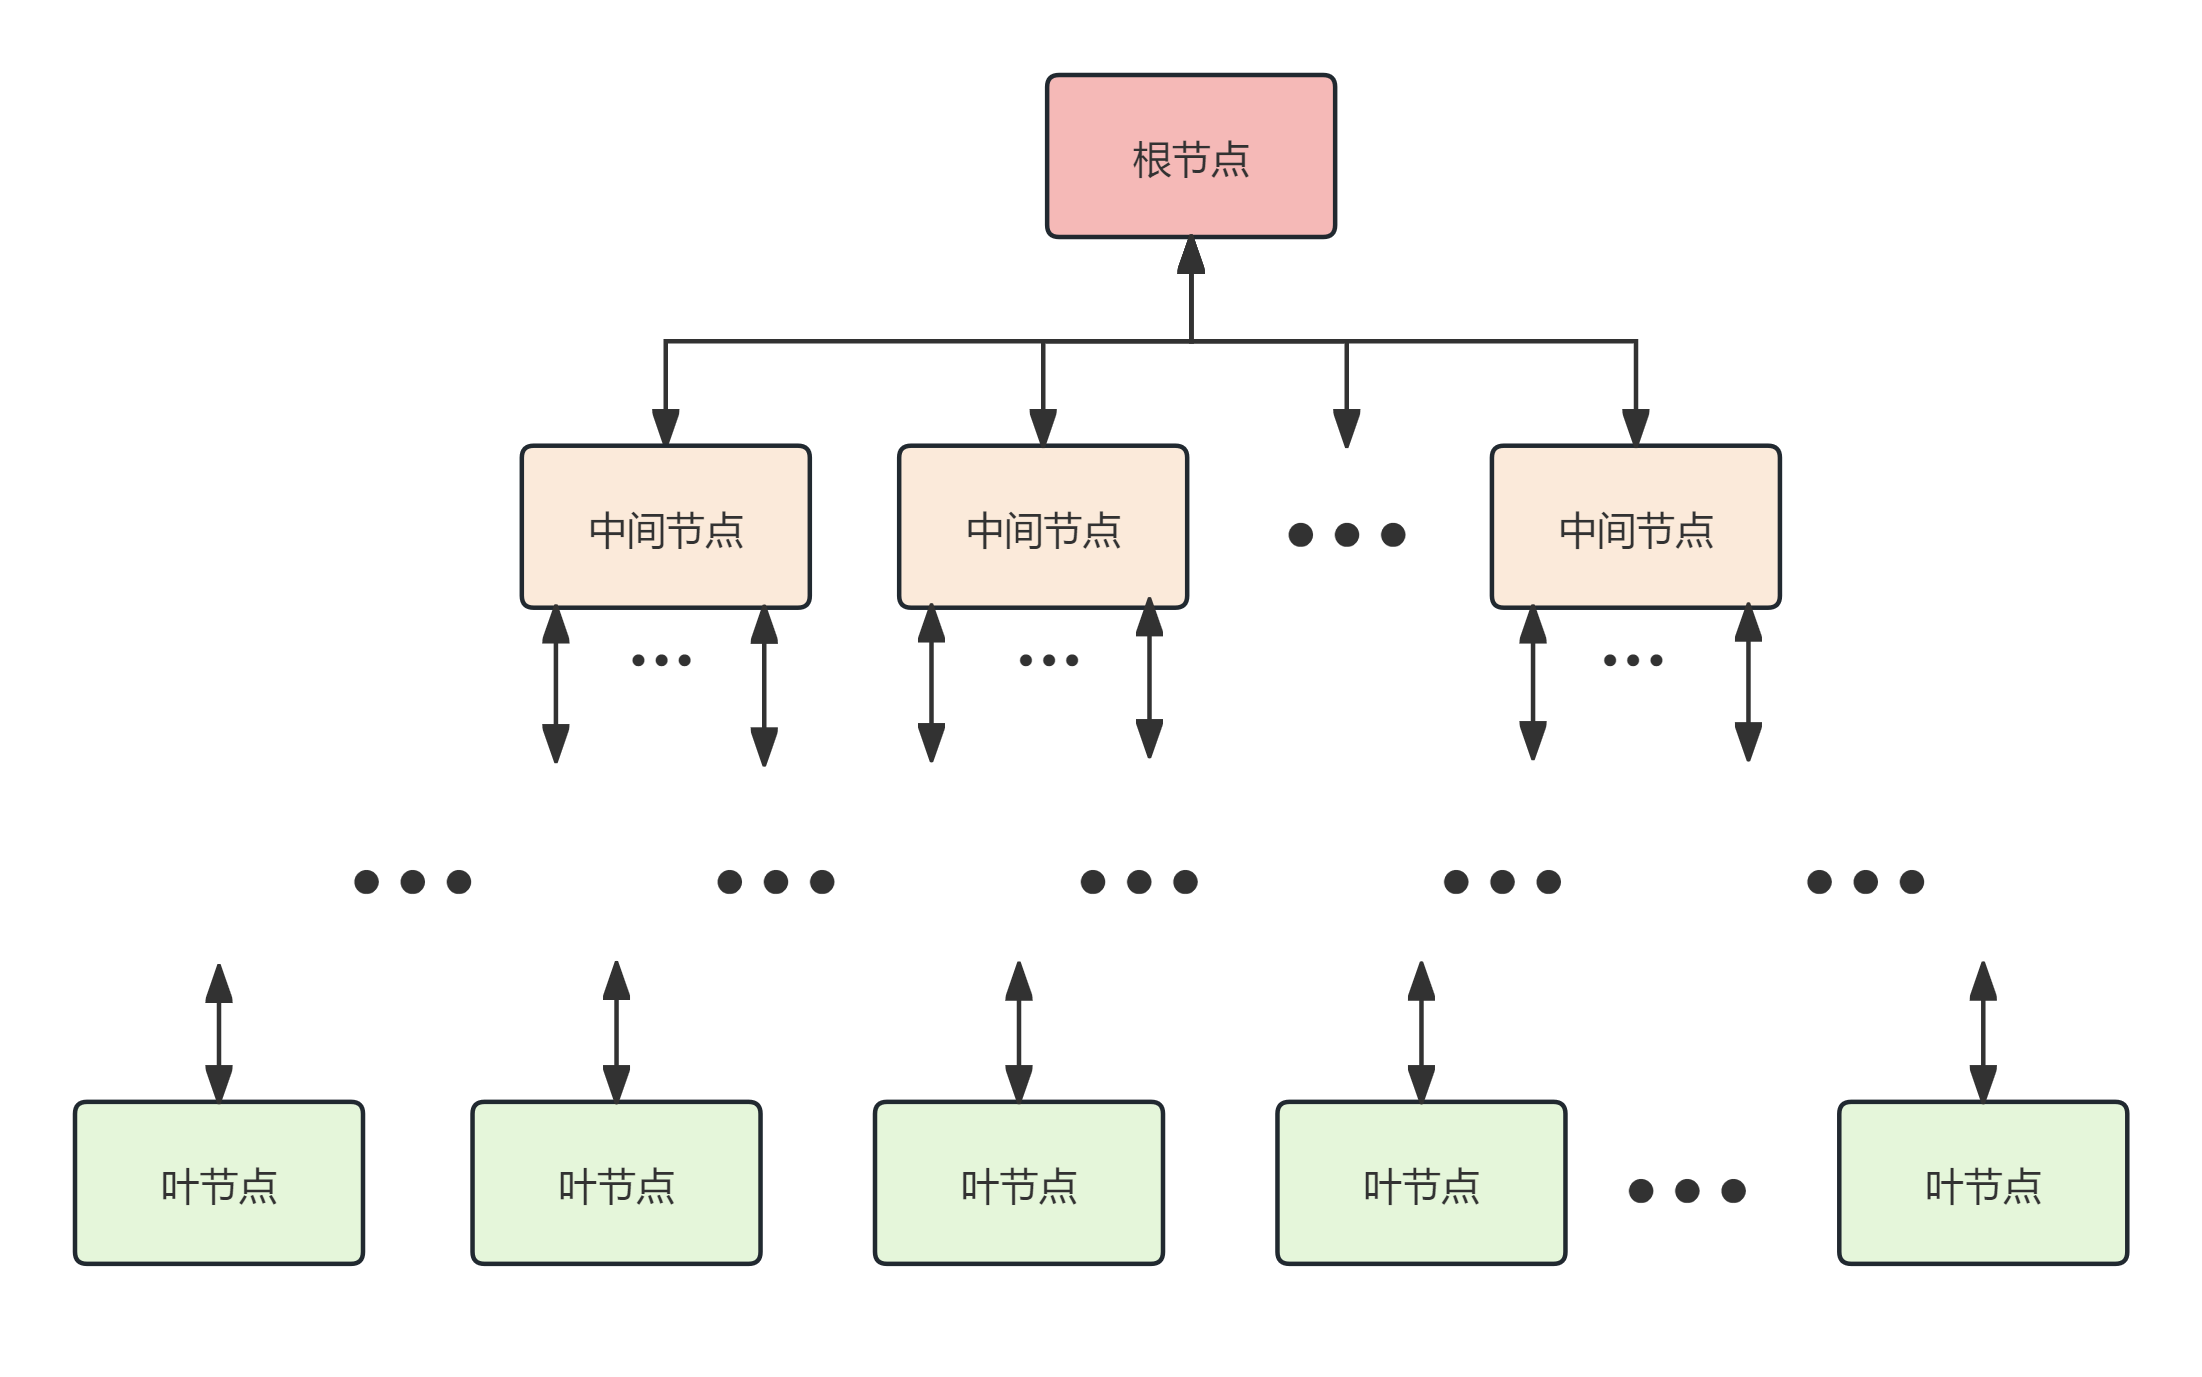
\includegraphics[width=0.6\linewidth]{rtmq/rtmq_nodes_and_leaves_structure}
\end{figure}

RTMQ架构主要用于基于FPGA或ASIC的兼具通用计算和高精度时序控制能力的微系统。系统的整体结构为树状结构,如图\ref{fig:rtmq_nodes_and_leaves_structure}所示,系统包含一个根节点,多个中间结点和多个叶节点;根节点通过网络、USB等方式与控制计算机相连。不同节点可位于同一PCB上,亦可位于不同PCB上。不同节点的时钟通过根节点进行对齐,各个节点都具有独立的控制输出和通用运算能力,能够分布式地完成实验的控制和信息处理。

\begin{figure}
    \centering
    \caption[RTMQ实时量子测控系统架构节点示意图]{RTMQ实时量子测控系统架构节点示意图\label{fig:rtmq_board_overal_structure}}
    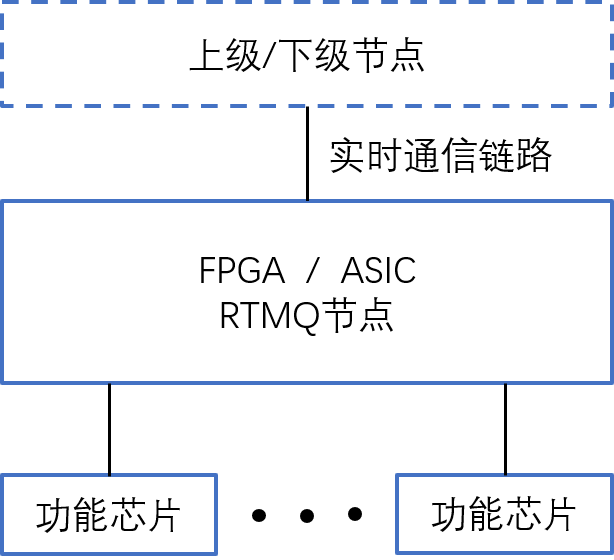
\includegraphics[width=0.4\linewidth]{rtmq/rtmq_board_overal_structure}
\end{figure}

各个节点都由测控硬件板卡构成,一般而言一个板卡具有如图\ref{fig:rtmq_board_overal_structure}所示的结构,板卡上的FPGA或ASIC包含一个RTMQ节点,RTMQ节点通过控制FPGA或ASIC的输入输出与数模/模数转换等各类功能芯片进行交互以实现所需功能,同时通过实时通信链路与其上级和下级节点连接。



\subsection[RTMQ实时量子测控系统架构的节点内部模块]{RTMQ实时量子测控系统架构的节点内部模块\label{section:rtmq_inner_module}}

\begin{figure}
    \centering
    \caption[RTMQ实时量子测控系统架构节点内部模块示意图]{RTMQ实时量子测控系统架构节点内部模块示意图\label{fig:rtmq_board_inner_structure}}
    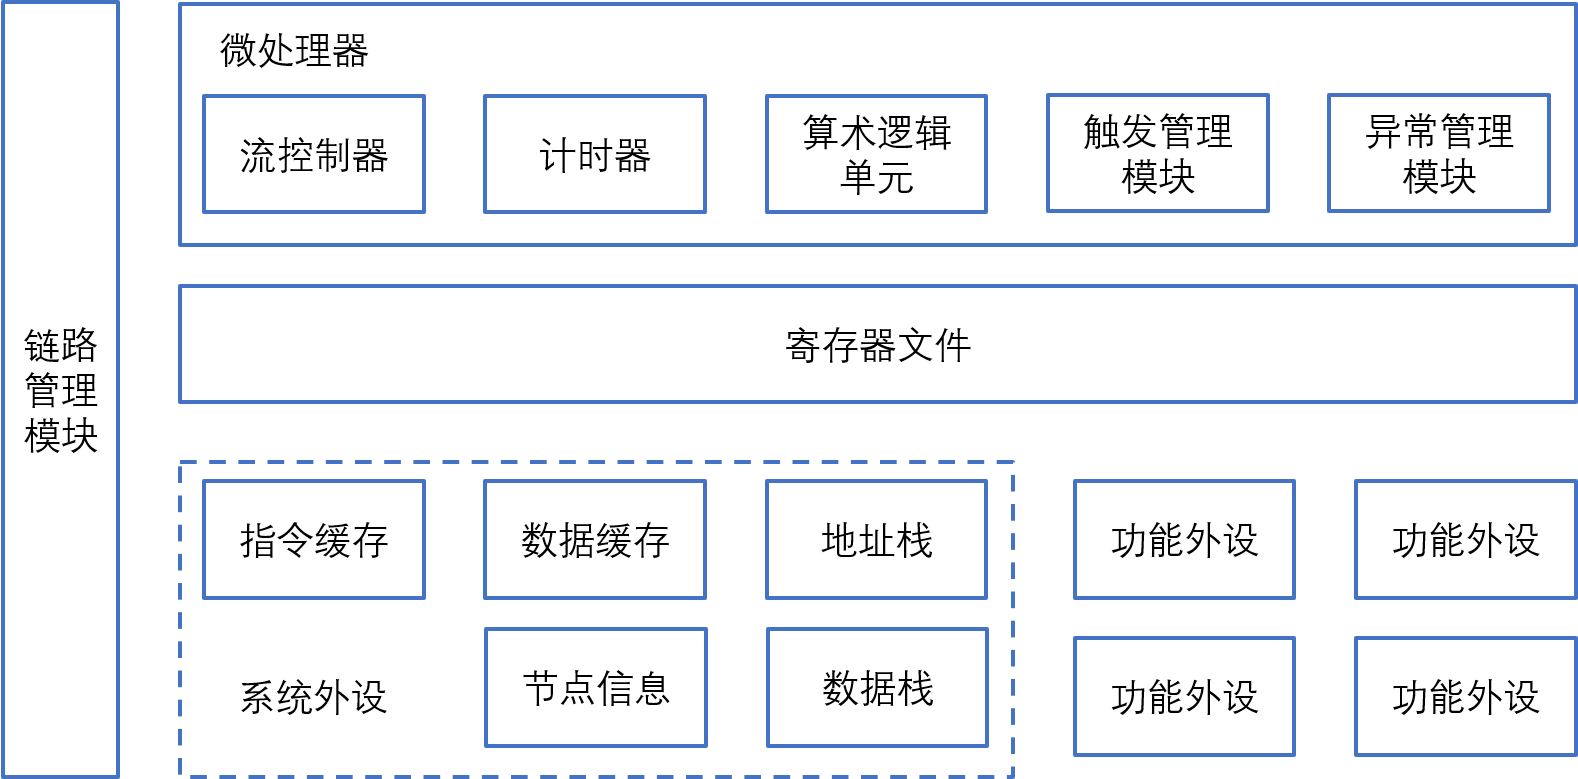
\includegraphics[width=1.0\linewidth]{rtmq/rtmq_board_inner_structure}
\end{figure}

一个RTMQ节点的内部模块如图\ref{fig:rtmq_board_inner_structure}所示,包含一个32位的微处理器、一个寄存器文件、一系列外设模块和一个链路管理模块。其中微处理器包含流控制器、计时器、异常管理模块、触发管理模块和算术逻辑单元5个子模块;寄存器文件包含多个寄存器;外设可分为系统外设和功能外设,系统外设包括指令缓存、数据缓存、节点信息只读存储器以及地址栈和数据栈,功能外设用于实现具体的逻辑或时序功能,可包含多个。

RTMQ架构中包含的微处理器可受指令控制进入挂起状态,而挂起状态可受计时器或触发管理模块的控制恢复正常运行,如此,微处理器的指令流便可以按一定的时间间隔对齐或与外部信号对齐。同时,节点中的系统外设和功能外设的行为受关联寄存器的读写控制,即微处理器的指令与系统各模块的功能和时序有严格的对应关系。因此,该架构可实现实时控制与通用计算在指令流层面的结合。
而配置指令插入中断的机制确保了节点对其下级节点的绝对控制,即使下级节点的微处理器处于挂起状态,依然不受影响。配置指令插入中断配合具有确定通信延迟的实时通信链路系统,即可实现时序确定的跨节点的即时反馈控制。
此外,RTMQ架构中每个节点都具有通用计算和时序控制能力,如此,大多数通用计算和时序生成都可以在叶节点或较近的中间结点完成,对于大规模系统不存在拥塞的问题,具有良好的可扩展性。RTMQ与之前离子阱领域常用的ARTIQ测控系统的对比如表\ref{tb:rtmq_artiq}所示,从对比中可见相较于ARTIQ,RTMQ在反馈延迟、分布式算力、节点自主性、ASIC兼容性、跨领域通用性等方面都有着巨大的优越性。

\begin{table}
    \centering
    \caption[RTMQ与ARTIQ对比]{RTMQ与ARTIQ对比\label{tb:rtmq_artiq}}    
    \begin{tabular}{L{5cm}|C{4cm}|C{4cm}}
        \toprule
        指标 & ARTIQ & RTMQ \\
        \midrule
        反馈延迟        & 十微秒 & 百纳秒 \\
        分布式算力      & × & √ \\
        节点自主性      & × & √ \\
        底端FPGA兼容性  & √ & √ \\
        ASIC兼容性      & × & √ \\
        二次开发能力    & √ & √ \\
        跨领域通用性    & × & √ \\
        \bottomrule
    \end{tabular}
\end{table}




% ============================================================================
% ============================================================================
% =======================      RTMQ Core       ===============================
% ============================================================================
% ============================================================================

\newpage
\section[RTMQ核心模块及其FPGA实现]{RTMQ核心模块及其FPGA实现}
% 在下面几小节中,我将介绍一些基本运算及外设模块的实现和使用。

RTMQ核心模块是一个专为实时量子计算设计的一个微处理器,具备完成强实时的数据处理能力,它在整个RTMQ测控系统重占据着十分核心的位置。如图\ref{fig:rtmq_core}所示,RTMQ的核心主要由三部分组成:流控制器、计时器、算术逻辑单元,它的输入及输出端口定义如表\ref{tb:rtmq_core}所示。本小节接下来的内容将介绍组成RTMQ核心模块的三个重要子模块流控制器、计时器、算术逻辑单元的逻辑功能和在Vivado中的FPGA实现。

% \textcolor{green}{具体内容描述待补充。}

\begin{table}
    \centering
    \caption[RTMQ核心模块端口定义]{RTMQ核心模块端口定义。IF:指令获取(Instruction Fetch)。\label{tb:rtmq_core}}    
    \begin{tabular}{L{2.5cm}L{4cm}|L{2.5cm}L{4cm}}
        \toprule
        \multicolumn{2}{c|}{Input} & \multicolumn{2}{c}{Output} \\
        \midrule
        Port & Define & Port & Define\\
        \hline
        cfg\_ins[31:0]  & 配置指令 & alu\_out[128:0] & 算术逻辑单元结果 \\
        clk             & 系统时钟 & f\_ftc & IF流水线获取标志 \\
        f\_cfg          & 配置指令覆盖标志 & f\_hld & 核心HOLD状态标志 \\
        f\_rsm          & 外部恢复标志 & if\_adr[31:0] & IF地址 \\
        if\_ins[31:0]   & IF输入 &  &  \\
        regfile[8191:0] & 寄存器文件 &  &  \\
        \bottomrule
    \end{tabular}
\end{table}


\begin{figure}
    \centering
    \caption[RTMQ核心微处理器的FPGA实现结构图]{RTMQ核心微处理器的FPGA实现结构图\label{fig:rtmq_core}}
    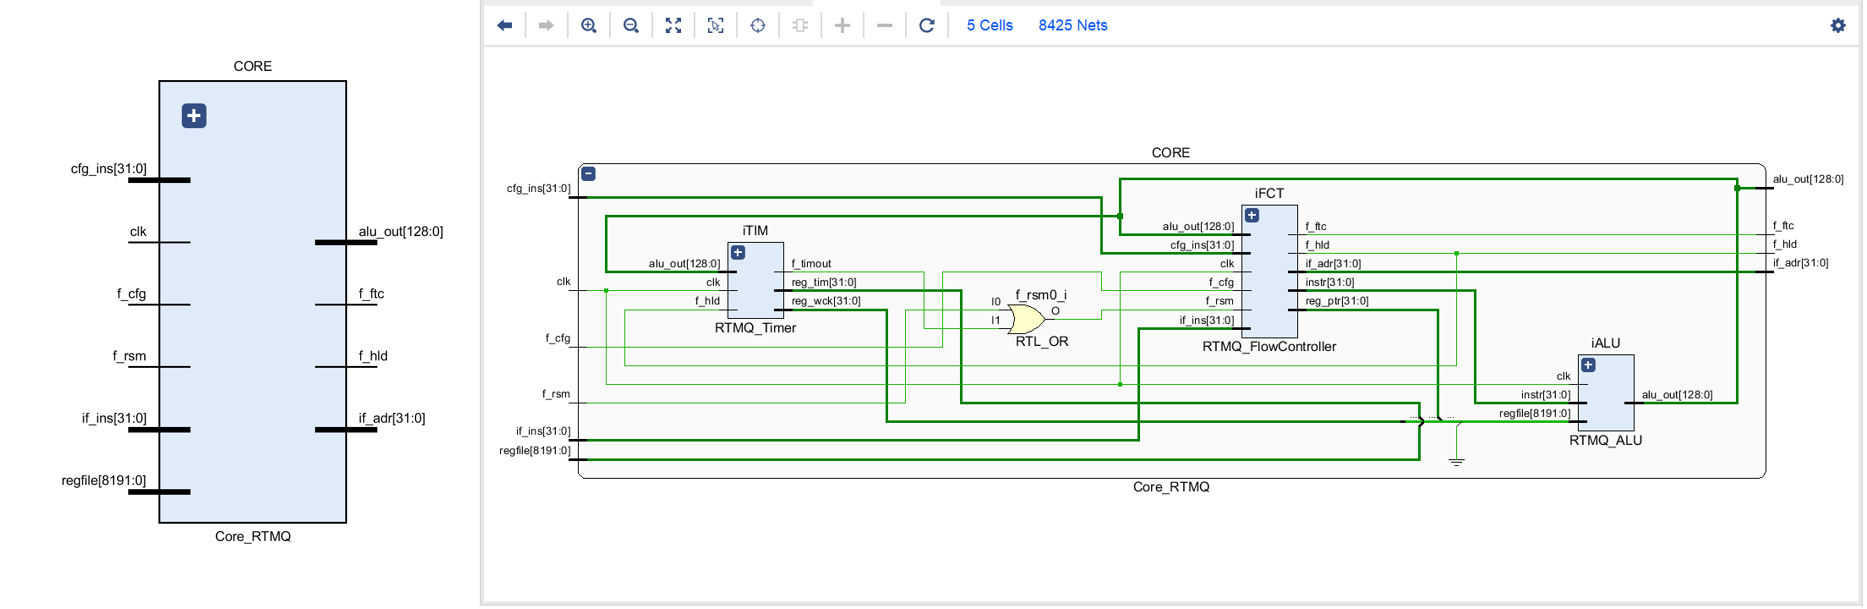
\includegraphics[width=1.0\linewidth]{rtmq/rtmq_core}
\end{figure}



\subsection[算术逻辑单元模块及其FPGA实现]{算术逻辑单元模块及其FPGA实现\label{section:rtmq_core_alu}}

算数逻辑单元模块式RTMQ微处理器核心的关键组成部分,它能够解析当前的输入指令进行运算处理并输出运算结果。如第\ref{section:rtmq_instruction_set}节所述,RTMQ算术逻辑单元的指令有两种,分别是A类指令和I类指令,两类指令的操作码及其含义分别如表\ref{tb:a_instructions}和表\ref{tb:i_instructions}所示,编码方案如表\ref{tb:instructions_code}所示。

该模块通过四级流水线处理了指令所要求的操作,将结果写入目的寄存器中同时给出一些辅助作用信号。
在第一级流水线中,对根据输入的regfile生成片选器选出R0和R1指向的操作数寄存器的数据用于后续的数据处理,同时将R0和R1的地址提取出来给出输出:alu\_r0a、alu\_r1a;如果是A类指令,则将R0和R1指向的操作数寄存器的数据片选结果保存到下级流水线使用;如果是I类指令,则不做特别操作。
在第二级流水线中,对R0和R1的数据根据不同的指令内容进行算术运算和逻辑运算的判断给出后续要执行的具体运算操作指示。
在第三级流水线中,根据不同指令情况进行运算,如算术比较、逻辑左右移位、算术左右移位、比特级翻转等,给出输出一些运算中间结果输出等待后续选用,同时给出目的寄存器地址输出:alu\_rda。
在第四级流水线中,根据A类或I类指令的具体需求给出相应的运算结果;对于A类指令给出模块运算结果和结果的掩码:alu\_res,alu\_msk;对于I类指令给出立即数的目的寄存器地址和操作目标段:imm\_rda、imm\_seg,并直接使用指令中的数据给出imm\_res。最终的算数逻辑单元模块输出结构alu\_out为:\{alu\_res, alu\_msk, alu\_rda, alu\_r0a, alu\_r1a,
imm\_res, imm\_rda, imm\_seg\}。

算数逻辑单元模块在Vivado中的FPGA实现结果如图\ref{fig:rtmq_alu}所示,其具体的接口定义如表\ref{tb:rtmq_alu}所示。

% \textcolor{green}{具体内容描述待补充。}


\begin{table}
    \centering
    \caption[RTMQ核心算术逻辑单元模块端口定义]{RTMQ核心算术逻辑单元模块端口定义\label{tb:rtmq_alu}}    
    \begin{tabular}{L{2.5cm}L{4cm}|L{2.5cm}L{4cm}}
        \toprule
        \multicolumn{2}{c|}{Input} & \multicolumn{2}{c}{Output} \\
        \midrule
        Port & Define & Port & Define\\
        \hline
        clk &  & alu\_out[128:0] & 算术逻辑单元结果 \\
        instr[31:0] & 当前指令 &  &  \\
        regfile[8191:0] & 寄存器文件 &  &  \\
        \bottomrule
    \end{tabular}
\end{table}


\begin{figure}
    \centering
    \caption[RTMQ核心算术逻辑单元模块的FPGA实现结构图]{RTMQ核心算术逻辑单元模块的FPGA实现结构图\label{fig:rtmq_alu}}
    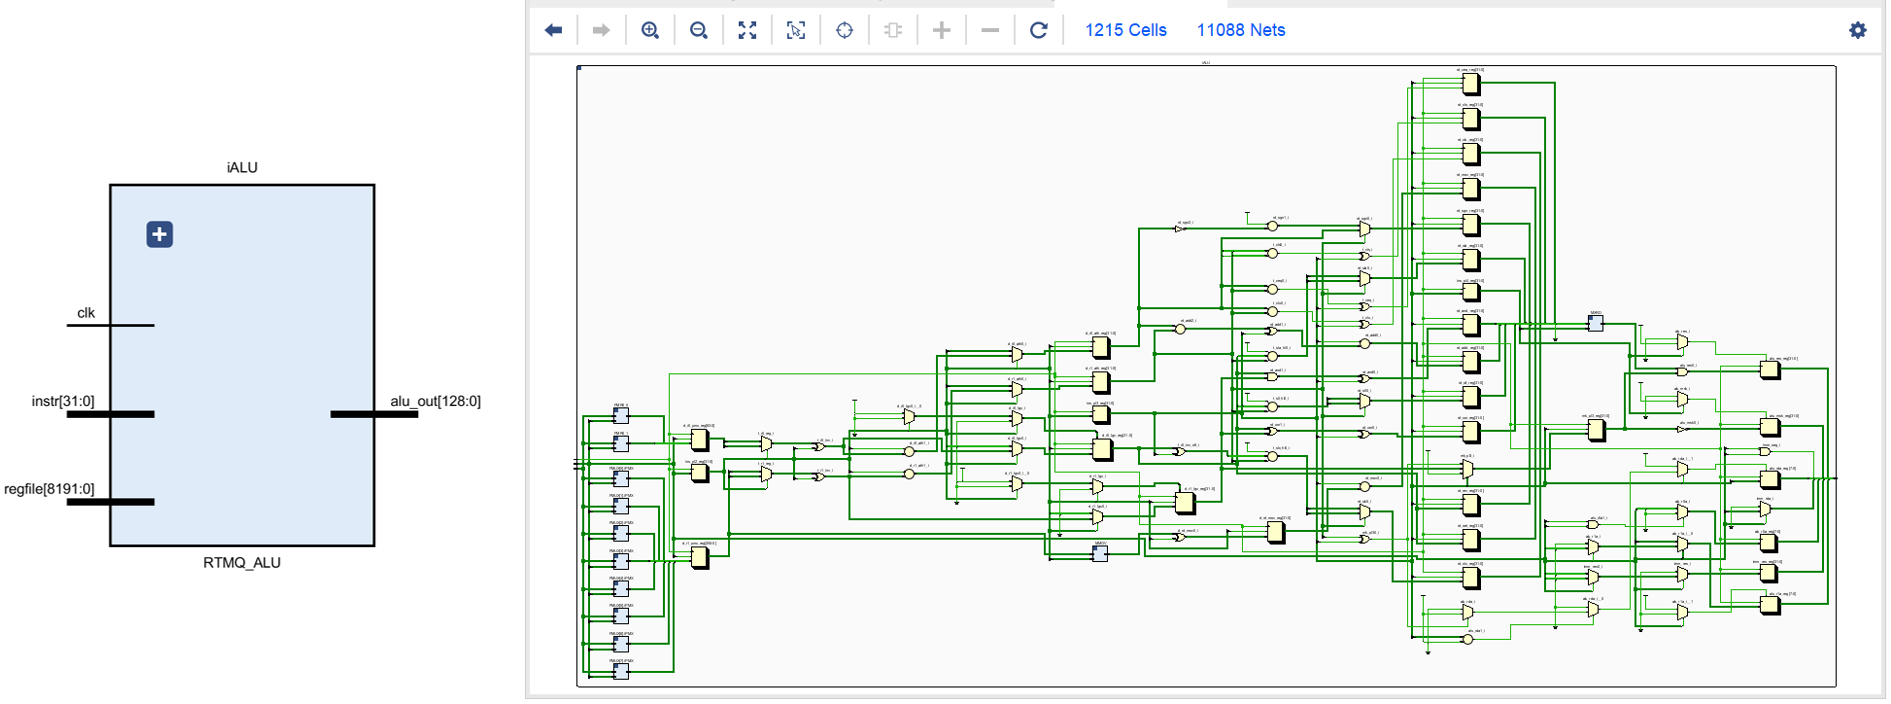
\includegraphics[width=1.0\linewidth]{rtmq/rtmq_alu}
\end{figure}




\subsection[流控制器模块及其FPGA实现]{流控制模块及其FPGA实现}

流控制器模块是确保RTMQ实时性的关键设计,也是其与经典CPU相比的不同所在。它接受ALU结果alu\_out、指令获取、外部恢复标志、配置指令及其覆盖标志等输入,给出regfile中的地址指针、获取指令地址、当前的指令内容、指令抓取标志、HOLD状态标志等输出。

RTMQ流控制器模块设计结构如图\ref{fig:rtmq_flow_controller_structure}所示,当配置指令覆盖标志、HOLD标志、指令中HOLD标志其中任何一个为“1”时,指令获取标志f\_ftc输出都为“0”(f\_nftc\_cmb为“1”)。
在f\_ftc不为零的情况下刷新一次指令获取流水线,同时指令获取地址if\_adr默认自动+1,另外也可以使用I类或A类指令对if\_adr进行赋值操作以实现指令跳转功能,这里I类指令只能实现较短的指令跳转,更大范围的指令跳转需要使用A类指令。
流控制器模块会根据不同情况选择输出不同的指令,共有四种情况:正常、配置、挂起、恢复。正常情况下输出的指令就是输入的指令,不做任何改变;如果进行了指令配置,那么输出的指令就是配置的指令内容;如果处于挂起状态,则输出指令为空;如果处于从HOLD状态中恢复的情况,则输出的指令为进入挂起状态前缓存的指令(进入HOLD状态时会对本应执行的指令进行缓存操作)。

对于寄存器文件中的地址指针reg\_ptr,默认情况下指针缓存ptr\_buf保持不变;如果进行了刷新操作,则将当前指针地址reg\_ptr存入指针缓存中;如果是进入挂起状态下,则将当前指针保存在缓存中。
默认会对指令地址进行3周期的缓存处理保存在ptr\_dly中,指针寄存器每次会读取ptr\_dly高位值,每访问一次就将高位的缓存指令推出,将新输入的指令推入低位;如果是刷新或挂起状态,则指针不变;如果是从挂起状态恢复,则指针重新恢复为挂起前的位置。

通过上述的逻辑,流控制器可以根据情况实现对ALU模块指令的选择输出、挂起和恢复等操作,且保证了每一条指令的执行、跳转、恢复等具有明确的操作时钟周期,可以用来满足量子测控系统对实时性的要求。流控制器模块在Vivado中的FPGA实现结果如图\ref{fig:rtmq_flow_control}所示,其具体的接口定义如表\ref{tb:rtmq_flow_control}所示。

% \textcolor{green}{具体内容描述待补充。}

\begin{figure}
    \centering
    \caption[RTMQ核心流控制器模块的设计结构图]{RTMQ核心流控制器模块的设计结构图\label{fig:rtmq_flow_controller_structure}}
    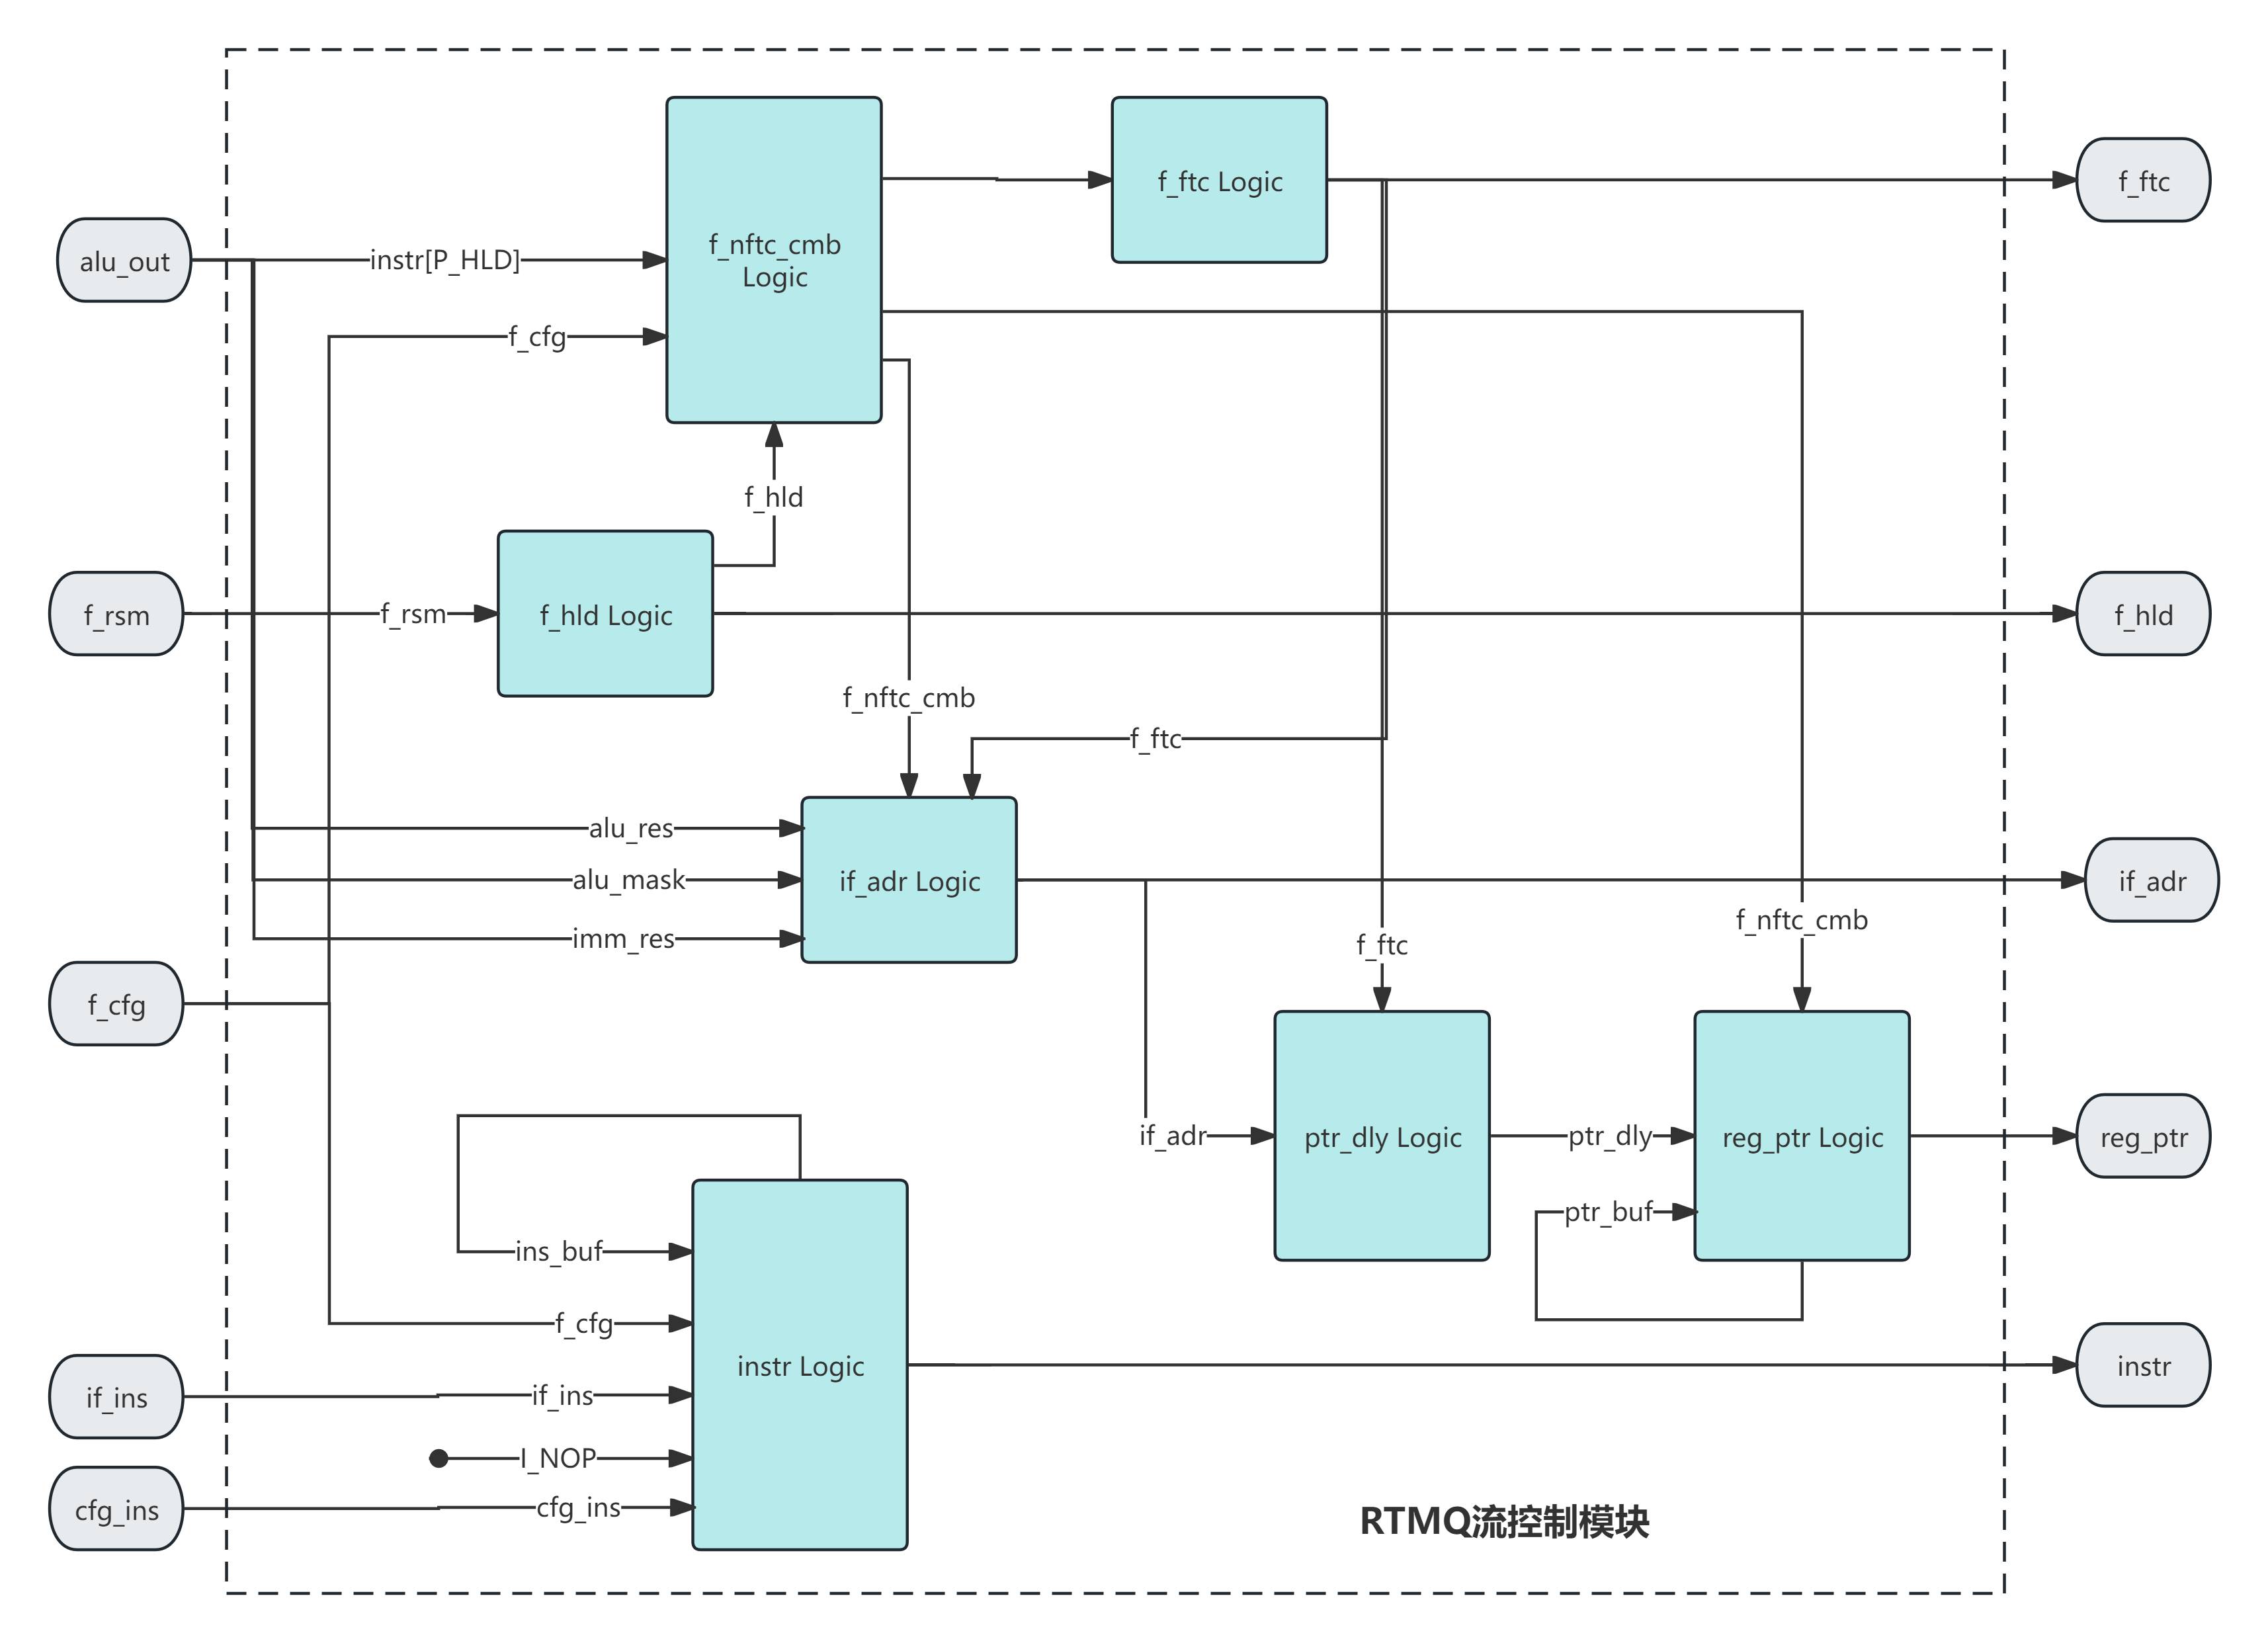
\includegraphics[width=1.0\linewidth]{rtmq/rtmq_flow_controller_structure}
\end{figure}

\begin{table}
    \centering
    \caption[RTMQ核心流控制器模块端口定义]{RTMQ核心流控制器模块端口定义\label{tb:rtmq_flow_control}}    
    \begin{tabular}{L{2.5cm}L{4cm}|L{2.5cm}L{4cm}}
        \toprule
        \multicolumn{2}{c|}{Input} & \multicolumn{2}{c}{Output} \\
        \midrule
        Port & Define & Port & Define\\
        \hline
        alu\_out[128:0] & 算术逻辑单元结果 & f\_ftc & IF流水线获取标志 \\
        cfg\_ins[31:0]  & 配置指令 & f\_hld & HOLD状态标志 \\
        clk             & 系统时钟 & if\_adr[31:0] & IF获取地址 \\
        f\_cfg          & 配置覆盖标志 & instr[31:0] & 当前指令内容 \\
        f\_rsm          & 外部恢复标志 & reg\_ptr[31:0] & regfile中的地址指针 \\
        if\_ins[31:0]   & IF输入 &  &  \\
        \bottomrule
    \end{tabular}
\end{table}

\begin{figure}
    \centering
    \caption[RTMQ核心流控制器模块的FPGA实现结构图]{RTMQ核心流控制器模块的FPGA实现结构图\label{fig:rtmq_flow_control}}
    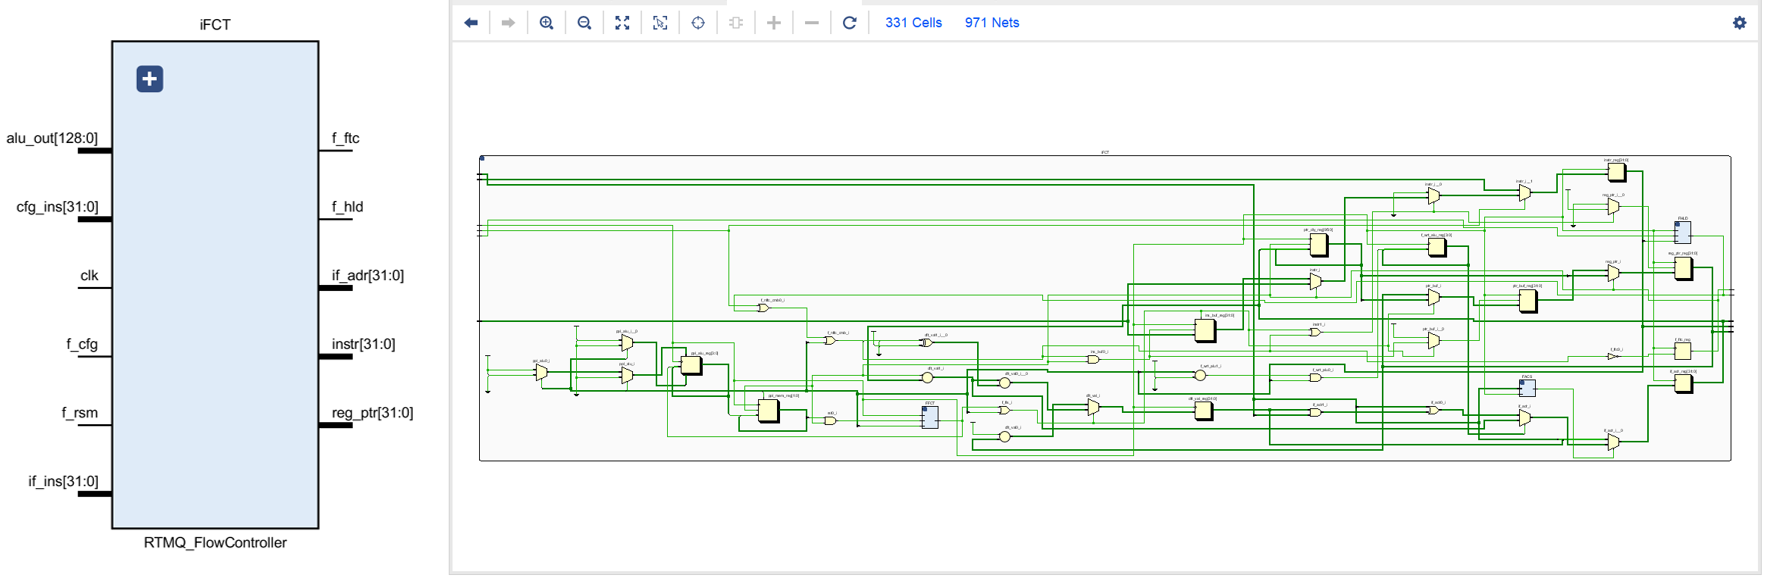
\includegraphics[width=1.0\linewidth]{rtmq/rtmq_flow_control}
\end{figure}





\subsection[计时器模块及其FPGA实现]{计时器模块及其FPGA实现}
计时器模块主要用于为RTMQ核心提供时间参考,它的输入是ALU结果alu\_out和挂起状态标志f\_hold,输出是系统以系统周期为单位的上电时间周期数[reg\_tim(墙时钟高段), reg\_wck(墙时钟低段)]和计时结束的恢复信号f\_timeout。
其结构如图\ref{fig:rtmq_timer_structure}所示,。计时器模块会保存从测控板上电开始的系统时间周期数以供其它模块获取和参考。另外也可以通过alu\_out的内容使用I类或者A类指令进行倒计时配置,配置完成后就会自动开始倒计时,计时结束时会给出一个可用于系统状态恢复的信号f\_timeout。

计时器模块在Vivado中的FPGA实现结果如图\ref{fig:rtmq_timer}所示,其具体的接口定义如表\ref{tb:rtmq_timer}所示。

\begin{figure}
    \centering
    \caption[RTMQ核心计时器模块的FPGA实现框图]{RTMQ核心计时器模块的FPGA实现框图\label{fig:rtmq_timer_structure}}
    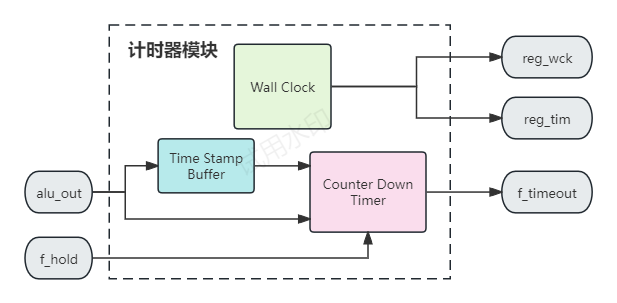
\includegraphics[width=1.0\linewidth]{rtmq/rtmq_timer_structure}
\end{figure}

\begin{table}
    \centering
    \caption[RTMQ核心计时器模块端口定义]{RTMQ核心计时器模块端口定义\label{tb:rtmq_timer}}    
    \begin{tabular}{L{2.5cm}L{4cm}|L{2.5cm}L{4cm}}
        \toprule
        \multicolumn{2}{c|}{Input} & \multicolumn{2}{c}{Output} \\
        \midrule
        Port & Define & Port & Define\\
        \hline
        alu\_out[128:0] & 算术逻辑单元结果 & f\_timeout& 计时结束标志,用于从HOLD状态恢复 \\
        clk             & 系统时钟 & reg\_tim[31:0] & 墙时钟高段,指示从系统上电起的周期数 \\
        f\_hld          & HOLD状态标志 & reg\_wck[31:0] & 墙时钟低段,指示从系统上电起的周期数 \\
        \bottomrule
    \end{tabular}
\end{table}

\begin{figure}
    \centering
    \caption[RTMQ核心计时器模块的FPGA实现结构图]{RTMQ核心计时器模块的FPGA实现结构图(Vivado)。\label{fig:rtmq_timer}}
    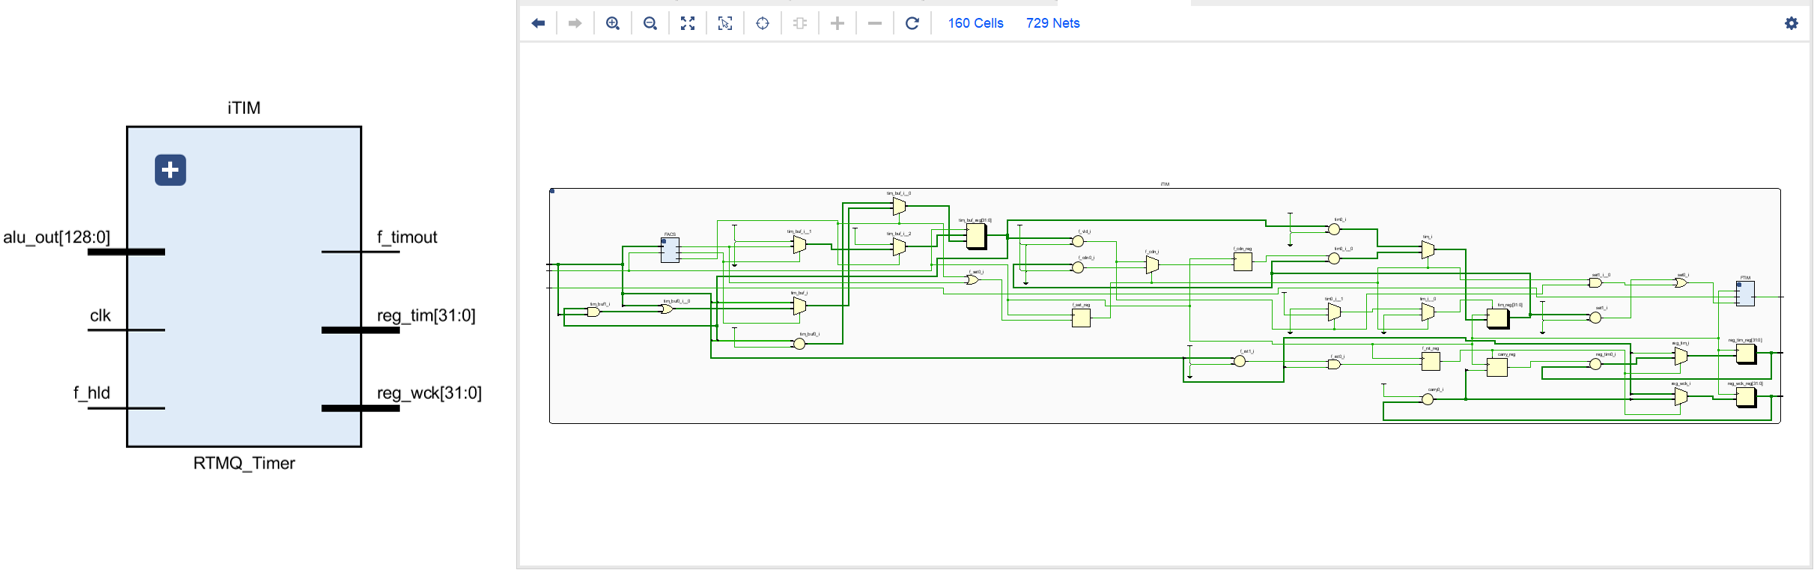
\includegraphics[width=1.0\linewidth]{rtmq/rtmq_timer}
\end{figure}











% \subsection[触发管理模块及其FPGA实现]{触发管理模块及其FPGA实现}

% \subsection[异常管理模块及其FPGA实现]{异常管理模块及其FPGA实现}






% ============================================================================
% ============================================================================
% ======================= RTMQ Instruction Set ===============================
% ============================================================================
% ============================================================================
\newpage
\section[RTMQ的指令集与时序控制结构描述]{RTMQ的指令集与时序控制结构描述}
RTMQ是专为可拓展实时量子计算而设计的核心微处理器,其配套设计了一种可用于实时控制和通用计算的指令集\cite[]{junhua03}。通过对寄存器的读写访问实现微系统架构中微处理器与其它逻辑功能模块之间的交互以及计时和流控制等操作构成基本的计时任务与非计时任务等与时序控制结构。该指令集与时序控制结构可以实现精确时序控制和通用计算能力在指令流层面的有机结合,其时序控制实现可准确至单个指令时钟周期。通用计算和流控制操作不会影响关键实时指令的执行时刻,能够适用于量子物理实验系统控制等对高精度时序控制和通用计算均有较高要求的领域。
接下来几小节将从指令的定义、指令的汇编语法、指令的编码、指令的执行逻辑、计时任务与非计时任务块结构等方面介绍RTMQ系统所采用的这种指令集与时序控制结构。

\subsection[RTMQ指令集描述]{RTMQ指令集描述\label{section:rtmq_instruction_set}}

与RTMQ架构配套的可用于实时控制和通用计算的指令集中指令包含以下部分:操作码、挂起标记、目标寄存器、操作数0和操作数1;指令集中的指令主要有两类:I类指令和A类指令,其中I类指令用于将操作数0或操作数1直接写入到目标寄存器,A类指令用于将操作数0和操作数1经过操作码指定的运算后的结果写入目标寄存器。I类指令的操作码及其含义如表\ref{tb:i_instructions}所示,A类指令的操作码及其含义如表\ref{tb:a_instructions}所示。

I类指令用于将立即数写入目标寄存器,仅使用1个立即数作为操作数;A类指令用于执行需要计算的操作,若操作数为寄存器,可在别名前加取反标记“!”,表示对该操作数取反后再进行计算;目标寄存器别名前亦可加取反标记,表示对运算结果取反后再写入目标寄存器;取反操作包括逻辑按位取反、数值反号以及特殊定义的取反操作,不同的指令使用不同的取反操作(逻辑按位取反操作即对操作数或计算结果的每一位进行逻辑取反;数值反号操作即对操作数或计算结果取二进制补码)。

当带有挂起标记的指令被执行后,执行指令的微处理器进入挂起状态,暂停指令的获取和执行。挂起标记H可为字符“H”或“-”;若为“H”,表示当前指令带有挂起标记,微处理器执行这条指令后进入挂起状态。
此外,指令集中的指令还包含跳转标记,其汇编指令的格式为:

\begin{align}
    OPC \qquad H \qquad F \qquad RD \qquad R0 \qquad R1
\end{align}

其中,OPC为操作码,H为挂起标记,F为跳转标记,RD为目标寄存器,R0为操作数0,R1为操作数1,操作数可为寄存器或立即数。每个寄存器对应一个别名和一个地址,分别用于在所述指令集的汇编指令和机器码中指代该寄存器。跳转标记F可为字符“F”或“-”;若为“F”,表示当前指令带有跳转标记,微处理器执行这条指令后将清空取指流水线。

\begin{table}
    \centering
    \caption[I类指令的操作码及其含义]{I类指令的操作码及其含义\label{tb:i_instructions}}
    \begin{tabular}{C{2cm}|C{12cm}}
        \toprule
        操作码 & 指令含义 \\
        \midrule
        LDL & 将指令携带的立即数载入目标寄存器的第19到第 0比特\\
        LDH & 将指令携带的立即数载入目标寄存器的第31到第20比特\\
        \bottomrule
    \end{tabular}
\end{table}

\begin{table}
    \centering
    \caption[A类指令的操作码及其含义]{A类指令的操作码及其含义\label{tb:a_instructions}}
    \begin{tabular}{C{1.3cm}|L{7.5cm}|C{1cm}|C{1cm}|C{2cm}}
        \toprule
        操作码 & 指令含义 & 操作数0取反 & 操作数1取反 & 结果取反 \\
        \hline
        \midrule
        ADD & 算术相加 RD = R0 + R1 & 数值反号 & 数值反号 & 数值反号 \\
        \hline
        AND & 按位逻辑与 RD = R0 \& R1 & 按位取反 & 按位取反 & 按位取反 \\
        \hline
        XOR & 按位逻辑或RD = R0 \| R1 & 按位取反 & 按位取反 & 按位取反 \\
        \hline
        CLU & 无符号小于,R0、R1视为无符号数,若R0 < R1则RD = 0xFFFFFFFF,否则RD = 0 & 数值反号 & 数值反号 & 按位取反 \\
        \hline
        CLS & 有符号小于,R0、R1视为有符号数,若R0 < R1则RD = 0xFFFFFFFF,否则RD = 0 & 数值反号 & 数值反号 & 按位取反 \\
        \hline
        CEQ & 等于,若R0 == R1则RD = 0xFFFFFFFF,否则RD = 0 & 数值反号 & 数值反号 & 按位取反 \\
        \hline
        SGN & 符号相乘,RD = R0 * sign(R1) & 数值反号 & 数值反号 & 不支持 \\
        \hline
        SNE & 条件赋值,当R1 < 0时RD = R0,否则RD不变 & 按位取反 & 数值反号 & 赋值条件改为R1 ≥ 0 \\
        \hline
        SMK & 掩码赋值,R1[i]为1时RD[i] = R0[i] ,否则RD[i]不变,Rx[i]代表Rx的第i比特 & 按位取反 & 按位取反 & 不支持 \\
        \hline
        MOV & 赋值,RD = R1 & 无R0 & 按位取反 & 运算结果+1\\
        \hline
        SLL & 逻辑左移,RD = R0 << R1[4:0],R1[4:0]代表R1的最低5比特,若R1 < 0 则为右移,左移时最低位填充R0的最低位,右移时最高位填充0; & 按位取反 & 数值反号 & 右移时最高位填充1 \\
        \hline
        SLA & 算术左移,RD = R0 << R1[4:0],若R1 < 0 则为右移,左移时最低位填充0,右移时最高位填充R0的最高位; & 按位取反 & 数值反号 & 左移时最低位填充1 \\
        \hline
        SLC & 循环左移,RD = R0 << R1[4:0],若R1 < 0 则为右移,移出端移出的比特填充到移入端;& 按位取反 & 数值反号 & 移出的比特按位取反后再填充 \\
        \hline
        REV & 反序,RD[i] = R0[31-i],将R0的二进制位顺序反向,将结果写入RD & 按位取反 & 无R1 & 不支持 \\
        \bottomrule
    \end{tabular}
\end{table}

\begin{table}
    \centering
    \caption[指令集的指令编码方案]{指令集的指令编码方案\label{tb:instructions_code}}
    \begin{tabular}{C{1cm}|C{1.5cm}|C{1.5cm}|C{2cm}|C{1cm}|C{5cm}}
    % \begin{tabular}{|c|c|c|c|c|c|}
        \toprule
         比特 & LDL & LDH & MOV & REV & 其它A类指令 \\
        \midrule
        31      & 1 & 1 & \multicolumn{3}{|c}{0} \\
        \hline
        30      & 1 & 0 & \multicolumn{3}{|c}{目标寄存器RD取反标记,为1则取反} \\
        \hline
        29      & \multicolumn{5}{|c}{挂起标记,为1则当前指令使得微处理器进入挂起状态} \\
        \hline
        28      & \multicolumn{5}{|c}{跳转标记,为1则微处理器清空从指令缓存取指的流水线} \\
        \hline
        27-24   & 立即数19-16位 & 0 & \multicolumn{3}{|c}{操作码} \\
        \hline
        23-16   & \multicolumn{5}{|c}{RD的地址} \\
        \hline
        15      & \multicolumn{2}{|c|}{立即数15位}  & 1 & 0 & 操作数R0立即数标记,为1表示R0为立即数 \\
        \hline
        14      & \multicolumn{2}{|c|}{立即数14位}  & 0 & 1 & R1立即数标记,为1表示R1为立即数 \\
        \hline
        13      & \multicolumn{2}{|c|}{立即数13位}   & 0 & \multicolumn{2}{|C{6cm}}{若R0为寄存器,则为取反标记,为1则取反;若R0为立即数,则为R0的第6位} \\
        \hline
        12      & \multicolumn{2}{|c|}{立即数12位}   & 操作数1取反标记,为1则取反 & 0 & 若R1为寄存器,则为取反标记;若R1为立即数,则为R1的第6位 \\
        \hline
        11-8    & \multicolumn{2}{|c|}{立即数11-8位}   & 0 & R0的地址 & 若R0为寄存器,则为其地址;若R0为立即数,则为其5-0位 \\
        \hline
        7-6     & \multicolumn{2}{|c|}{立即数7-6位}   & R1地址 & 0 & 若R0为寄存器,则为其地址;若R0为立即数,则为其5-0位\\
        \hline
        5-0     & \multicolumn{2}{|c|}{立即数5-0位}   & R1地址 & 0 & 若R1为寄存器,则为其地址;若R1为立即数,则为其5-0位 \\
        \bottomrule
    \end{tabular}
\end{table}


本文涉及的RTMQ为32位系统,其寄存器的位宽为32位,因此相应指令集的指令编码长度也为32位。指令集的指令编码方案如表\ref{tb:instructions_code}所示,大体有五类情况:LDL、LDH、MOV、REV及其它A类指令。几类情况的共同点为[29-28]位分别为挂起和跳转标志位以及[23-16]位为RD地址,其余各位的编码根据具体的操作而有所不同。
其中,LDL和LDH为I类指令,两者的区别主要在于载入立即数位数的不同。其中LDL会将指令携带的立即数载入目标寄存器的第19到第0比特(20位),而LDH会将指令携带的立即数载入目标寄存器的第31到第20比特(12)位。在A类指令编码中有两个特殊的指令MOV和REV,与其余A类指令每次同时操作R0和R1两个操作数不同,这两个指令操作对象仅为一个操作数(R0或R1)。

第\ref{section:rtmq_structure}节中提出的RTMQ微系统架构中包含响应指令集相关操作的寄存器的读、写访问的功能逻辑模块。当RTMQ中某一寄存器作为A类指令的操作数被读取时,与其关联的上述功能逻辑模块执行响应读取访问的逻辑功能。当某一寄存器作为A类指令或I类指令中的LDL指令的目标寄存器被写入时,与其关联的上述功能逻辑模块执行响应写入访问的逻辑功能。

如第\ref{section:rtmq_inner_module}节所述,在RTMQ微系统架构中也包含与寄存器TIM关联的计时器模块与指令集相配合。具体来说,当TIM寄存器被写入时,计时器模块激活倒计时,倒计时的起始时间计数为TIM寄存器的写入值;每个系统时钟周期时间计数减1,直到为0时停止倒计时;倒计时结束时,若该微系统架构中的微处理器处于挂起状态,则解除该挂起状态。
此外,RTMQ中包含别名为NUL、地址为0的寄存器,定义为空寄存器,对空寄存器的写入操作不产生任何效果,而其读取值恒为0。空指令“NOP H F”定义为“ADD H F NUL NUL NUL”,挂起标记H和跳转标记F可根据需要设定,除此之外空指令不产生任何其它效果。

\subsection[RTMQ时序控制结构:计时任务块与非计时任务块]{实例:计时任务块与非计时任务块}

基于第\ref{section:rtmq_instruction_set}节中所述的指令集和RTMQ计时器模块的逻辑功能,可以定义结合精确时序控制和通用计算的程序结构,称为计时任务块,其两种等价结构如表\ref{tb:timed_program1}和表\ref{tb:timed_program2}所示。在实际实验应用中会存在与所述计时任务块在功能上等价的其它程序结构,包括但不限于将挂起标记H向上一条指令或下一条指令移动、利用其它指令写入TIM寄存器等等情况。

\begin{table}
    \centering
    \caption[计时任务块结构]{计时任务块结构\label{tb:timed_program1}}
    \begin{tabular}{C{7cm}|C{7cm}}
        \toprule
        若T为寄存器 & 若T为立即数 \\
        \midrule
        NOP - -& LDH - - TIM T \\
        MOV - - TIM T & LDL - - TIM T \\
        \dots  & \dots \\
        (一条或多条其它指令) & (一条或多条其它指令) \\
        NOP H - & NOP H -\\
        \bottomrule
    \end{tabular}
\end{table}

\begin{table}
    \centering
    \caption[计时任务块另一等价结构]{计时任务块另一等价结构\label{tb:timed_program2}}
    \begin{tabular}{C{7cm}|C{7cm}}
        \toprule
        若T为寄存器 & 若T为立即数 \\
        \midrule
        NOP H -& NOP H -\\
        NOP - -& LDH - - TIM T\\
        MOV - - TIM T & LDL - - TIM T\\
        \dots  & \dots \\
        (一条或多条其它指令) & (一条或多条其它指令)\\
        \bottomrule
    \end{tabular}
\end{table}

若在程序中有大计算量的通用计算存在或有等待外触发等执行时间可能不确定的需求,可定义非计时任务块结构,其结构如表\ref{tb:untimed_program}所示。在实际实验应用中也会存在与“MOV - - TIM NUL”等价的其它激活计时器的短时间倒计时的方式,包括但不限于使用“ADD - - TIM NUL NUL”、“LDL - - TIM 0”等功能上等价的指令以及对初始时间计数的调整。

\begin{table}
    \centering
    \caption[非计时任务块结构]{非计时任务块结构\label{tb:untimed_program}}
    \begin{tabular}{C{14cm}}
        \toprule
        NOP H -\\
        (一条或多条其它指令)\\
        MOV - - TIM NUL \\
        \bottomrule
    \end{tabular}
\end{table}










% ============================================================================
% ============================================================================
% ======================     RTMQ Link System   ==============================
% ============================================================================
% ============================================================================
\newpage
\section[RTMQ节点间的实时通信链路系统描述]{RTMQ节点间的实时通信链路系统描述}

RTMQ实时量子测控系统架构具有强大的可拓展性,不同板卡节点之间可以实现完全的实时通信,这种通信的实现依赖于一种专门设计的链路系统。
该链路系统中,所有节点与其上级、下级节点之间具有统一、固定且较短的通信延迟,适用于实时控制的场景;并且链路中除了可传递数据,亦可传递指令,方便上级节点对下级节点进行实时的控制,以实现更为复杂的交互功能。

\subsection[RTMQ节点间的实时通信链路系统]{RTMQ节点间的实时通信链路系统}
如第\ref{section:rtmq_architecture}节所述,由RTMQ节点组成的硬件系统呈树状结构拓展,节点分为根节点、中间结点和叶节点三类。根节点和中间结点拥有一个或多个与其直接相连的下级节点,中间结点和叶节点拥有一个与其直接相连的上级节点。
该链路系统中节点间直接通信的物理链路协议为具有固定通信延迟、固定最小通信单元长度的双向点对点通信协议,如UART或SPI。

RTMQ节点间的通信以帧为单位,帧包含魔术字、跳转数、帧类型和载荷4个数据域。其中魔术字用于验证当前帧的有效性;跳转数用于指示当前帧可被转发的次数;帧类型可为数据帧或指令帧,用于指示当前帧的载荷类型;载荷为当前帧所携带的有效信息,根据当前帧的帧类型,载荷可被接收该帧的节点解析为数据或指令。从一个节点向其下级节点发送或转发的帧称为下行帧;从一个节点向其上级节点发送或转发的帧称为上行帧。

每个RTMQ节点包含一个链路管理模块,用于实现节点间的通信逻辑功能,其功能如表\ref{tb:rtmq_link_module}所示,具体功能的实现依赖链路管理模块的若干子模块。如图\ref{fig:rtmq_link_module}所示,物理链路子模块有两种,记为上级节点通信物理链路0模块和下级节点通信物理链路x模块。物理链路0模块实现与上级节点通信的物理链路逻辑,此类模块每个节点仅有一个;物理链路x模块实现与下级节点x通信的物理链路逻辑,此类模块的个数与当前节点所拥有的下级节点的数目相同。
下级节点收发逻辑子模块用于处理来自上级节点的下行帧,或向上级节点发送上行帧,以实现表\ref{tb:rtmq_link_module}中功能F1、F2、F6、F7,它与物理链路0模块相连。下级节点x收发逻辑子模块用于处理来自下级节点x的上行帧,或向下级节点x发送下行帧,以实现所述功能F3-F7,它与物理链路x模块相连。广播逻辑子模块用于向多个指定的下级节点广播下行帧,以实现所述功能F4、F6,它与所有下级节点收发逻辑模块相连。下行帧转发逻辑子模块用于来自上级节点的下行帧的向下广播转发,以实现所述功能F6,它与上级节点收发逻辑模块及广播逻辑模块相连。
上行帧转发逻辑子模块用于向上级节点转发来自指定下级节点的上行帧,以实现所述功能F7,它与上级节点收发逻辑模块及所有下级节点收发逻辑模块相连。


\begin{table}
    \centering
    \caption[链路管理模块通信逻辑功能及其子模块对应]{链路管理模块通信逻辑功能及其子模块对应\label{tb:rtmq_link_module}}
    \begin{tabular}{C{1.5cm}|C{5.5cm}|C{6cm}}
        \toprule
        功能 & 功能内容 & 实现涉及的子模块\\
        \midrule
        F1 & 向上级节点发送上行帧 & 下级节点收发逻辑子模块\\
        \hline
        F2 & 接收并解析来自上级节点的下行帧 & 下级节点收发逻辑子模块\\
        \hline
        F3 & 向指定的下级节点发送下行帧 & 下级节点x收发逻辑子模块\\
        \hline
        F4 & 同时向多个指定的下级节点广播同一下行帧 & 下级节点x收发逻辑子模块、广播逻辑子模块\\
        \hline
        F5 & 接收并解析来自各下级节点的上行帧 & 下级节点x收发逻辑子模块\\
        \hline
        F6 & 同时向多个指定的下级节点广播转发来自上级节点的下行帧 & 下级节点收发逻辑子模块、下级节点x收发逻辑子模块、广播逻辑子模块、下行帧转发逻辑子模块\\
        \hline
        F7 & 向上级节点转发来自指定的下级节点的上行帧 & 下级节点收发逻辑子模块、下级节点x收发逻辑子模块、上行帧转发逻辑子模块\\
        \bottomrule
    \end{tabular}
\end{table}


\begin{figure}
    \centering
    \caption[链路管理模块内部逻辑结构图]{链路管理模块内部逻辑结构图\label{fig:rtmq_link_module}}
    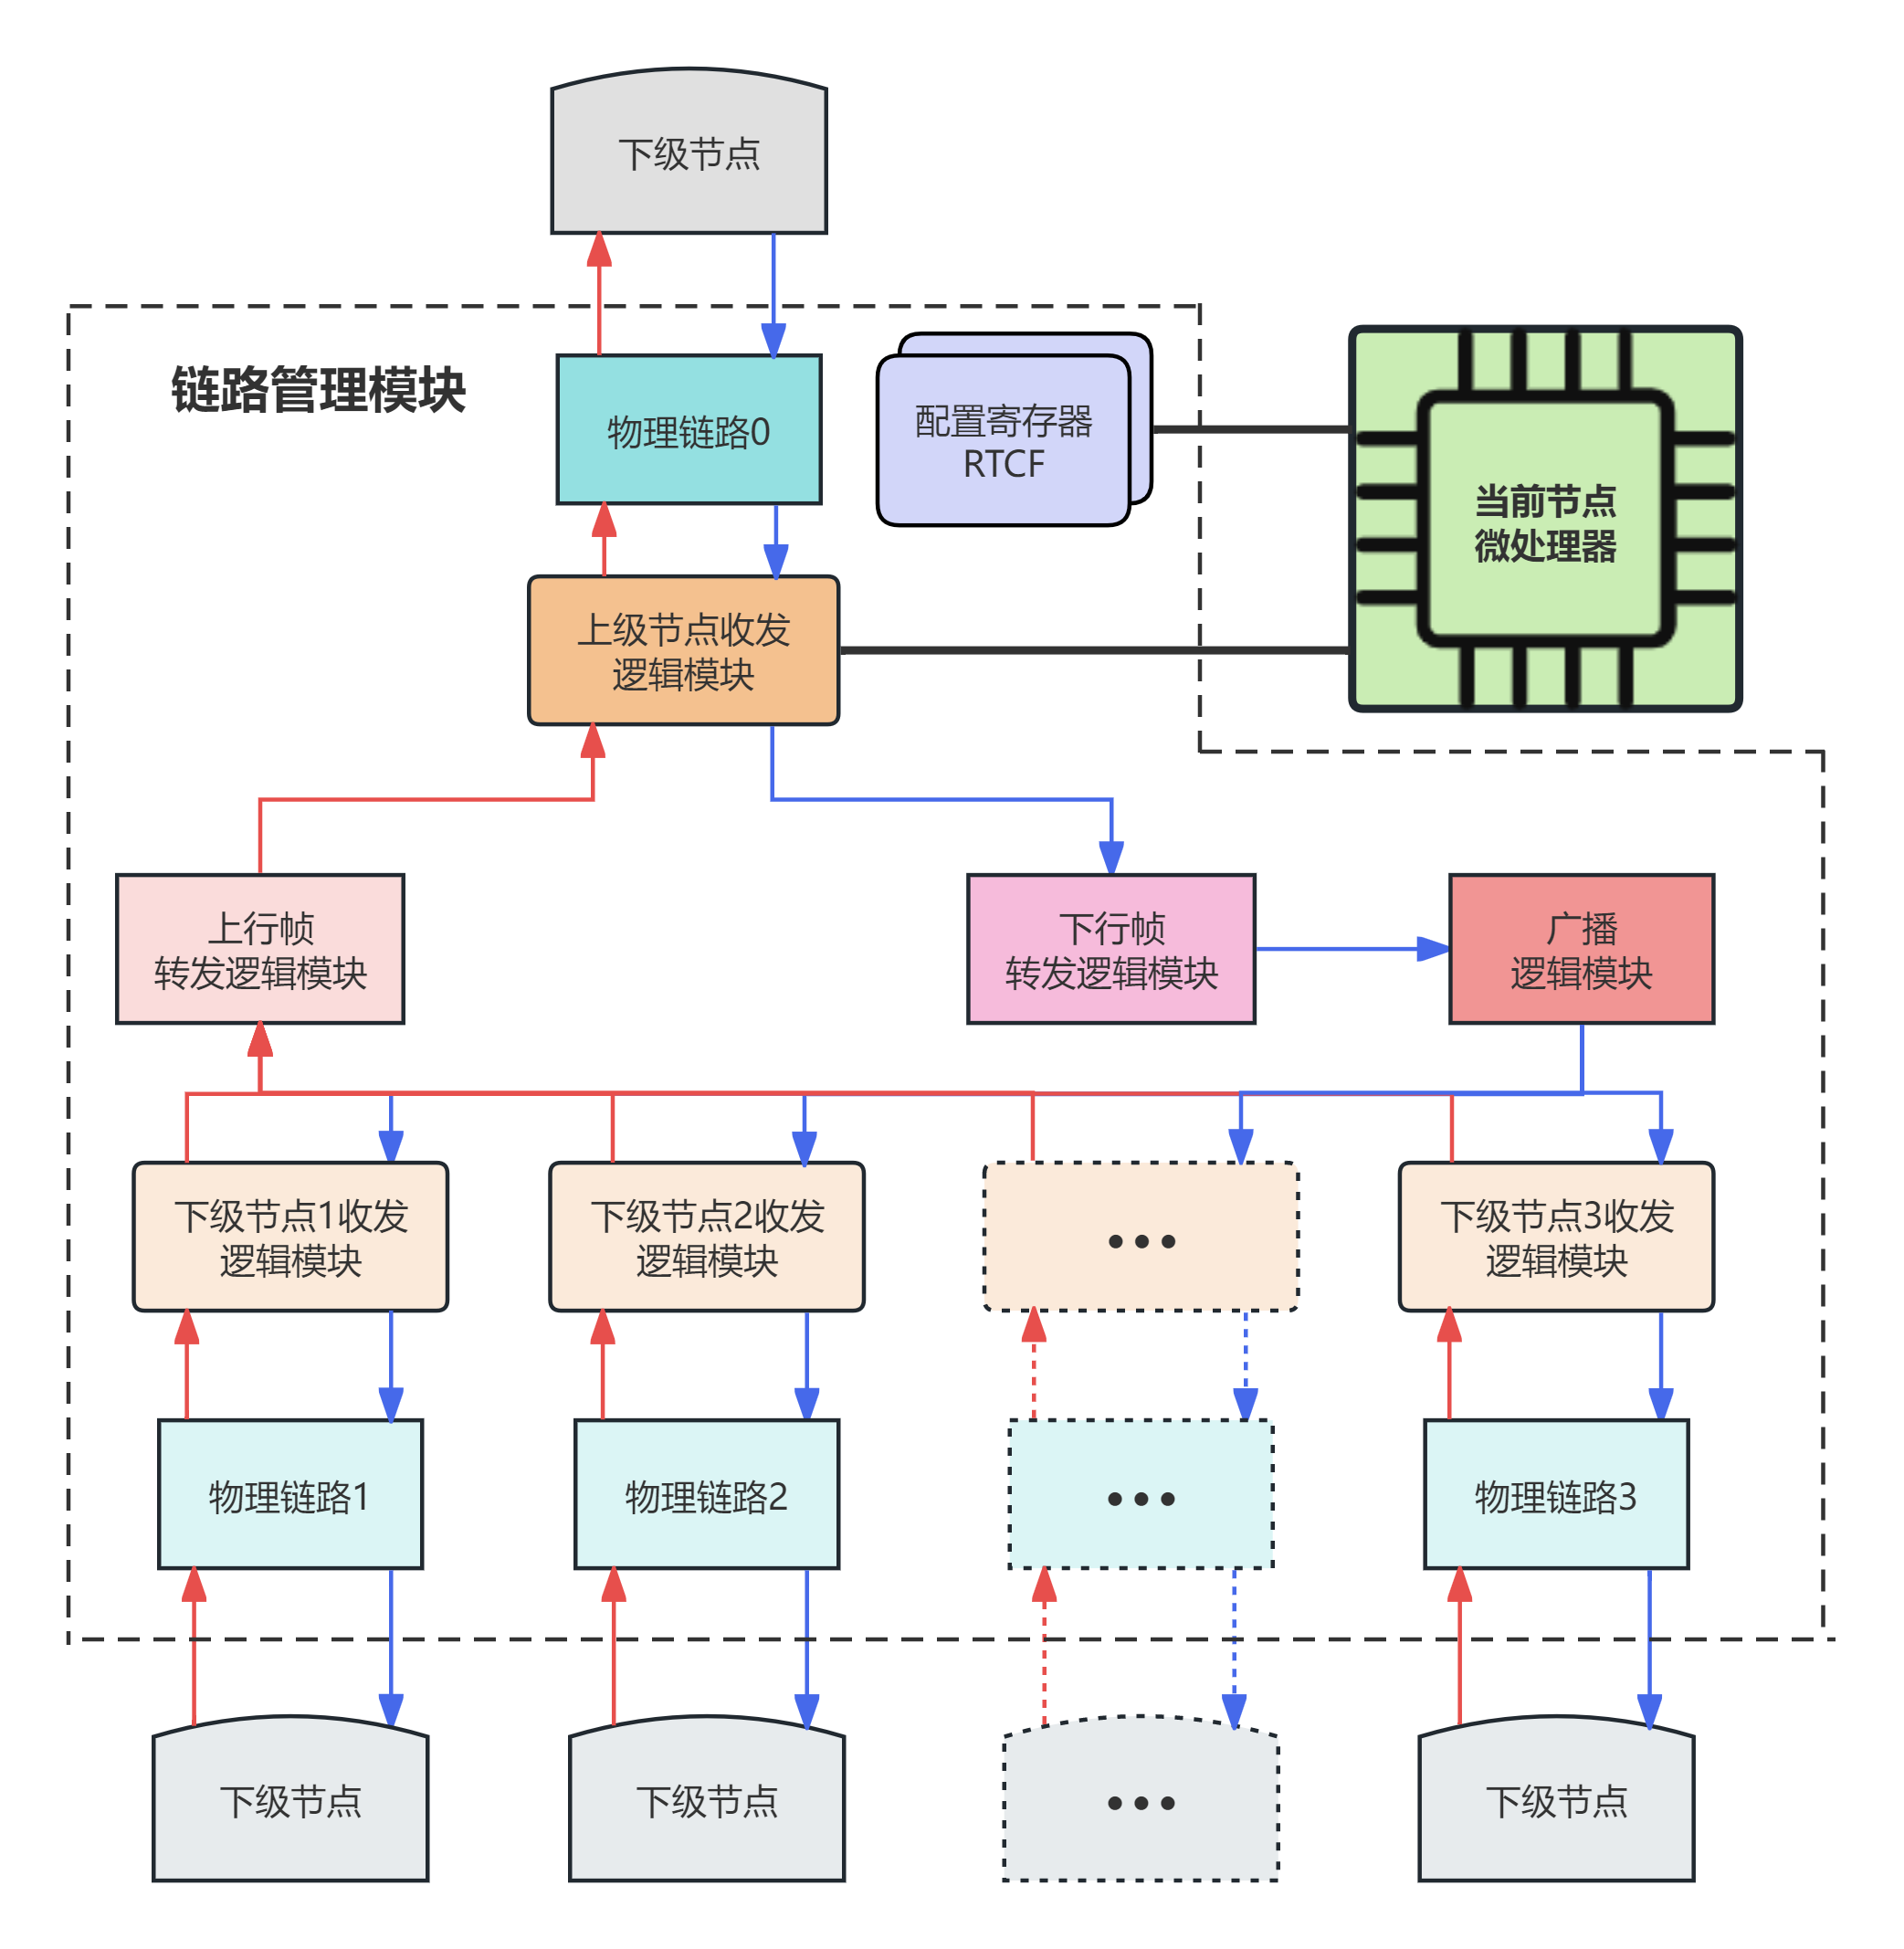
\includegraphics[width=1.0\linewidth]{rtmq/rtmq_link_module}
\end{figure}


每个节点的链路管理模块都关联以下寄存器:配置寄存器RTCF、广播寄存器RTBC、上行链路寄存器RTD0、下行链路寄存器RTD1、RTD2、……、RTDx。向以上寄存器写入数据,能够调控链路管理模块的不同逻辑功能,从这些寄存器读取数据,可以获取链路管理模块从链路系统中接收到的数据,以及其它相关信息。每个节点都包含一个RTMQ微处理器,微处理器可以通过指令读取或写入与链路管理模块关联的寄存器,以控制其执行各项逻辑功能。

其中配置寄存器RTCF的配置功能如表\ref{tb:rtmq_link_rtcf}所示,它有C1-C5五个可配置项。其中,C1为上行帧发送数据源选择配置项,它可以配置为来自RTD0或转发来自下级节点x的上行帧;C2为下行帧广播数据源选择配置项,它可以配置为来自RTBC或转发来自上级节点的下行帧;C3.x为向下级节点x发送的下行帧数据源选择配置项,它可以配置为来自RTDx或来自广播逻辑模块;C5负责配置各物理链路0模块、物理链路x模块运行所需的其它参数,它可以配置多个参数,包括但不限于通信链路的时钟分频系数。而从RTCF中读取数据可获得的信息可根据实际需要确定,包括各物理链路模块的占用状态等等。

\begin{table}
    \centering
    \caption[配置寄存器RTCF的配置功能表]{配置寄存器RTCF的配置功能表\label{tb:rtmq_link_rtcf}}
    \begin{tabular}{C{1.5cm}|C{5.5cm}|C{6cm}}
        \toprule
        配置 & 功能内容 & 配置可选项\\
        \midrule
        C1 & 上行帧发送数据源选择 & 选项P1.0:来自RTD0;
        选项P1.x:转发来自下级节点x的上行帧;
        \\
        C2 & 下行帧广播数据源选择 & 选项P2.0:来自RTBC;
        选项P2.1:转发来自上级节点的下行帧;
        \\
        C3.x & 向下级节点x发送的下行帧数据源选择 & 选项P3.x.0:来自RTDx;
        选项P3.x.1:来自广播逻辑模块;
        \\
        C4 & 当前节点发起帧的帧类型和跳转数 & —— \\
        C5 & 各物理链路0模块、物理链路x模块运行所需的其它参数 & 可包含多个参数,包括通信链路的时钟分频系数等等;\\
        \bottomrule
    \end{tabular}
\end{table}

其中广播寄存器RTBC的功能为向所有RTCF中的配置C3.x被设定为选项P3.x.1的下级节点x广播发送下行帧,该模块写入操作时激活广播逻辑模块,该功能的启用需要RTCF的配置C2设定为选项P2.0(来自RTBC);该下行帧的帧类型和跳转数由RTCF中的配置C4确定,其载荷为该写入操作向RTBC写入的数据。从RTBC读取数据,可获得的信息可根据实际需要确定。

其中上行链路寄存器RTD0的功能为向上级节点发送上行帧,该模块写入操作时激活上级节点收发逻辑模块,该功能的启用需要RTCF的配置C1设定为选项P1.0(来自RTD0);该上行帧的帧类型和跳转数由RTCF中的配置C4确定,其载荷为该写入操作向RTD0写入的数据。从RTD0读取数据,可按接收顺序获得来自上级节点且跳转数为0的下行数据帧的载荷。

其中任一下行链路寄存器RTDx的功能为向下级节点x发送下行帧,该模块写入操作时激活下级节点x收发逻辑模块,该功能的启用需要RTCF的配置C3.x设定为选项P3.x.0(来自RTDx);该下行帧的帧类型和跳转数由RTCF中的配置C4确定,其载荷为该写入操作向RTDx写入的数据。从任一RTDx读取数据,可按接收顺序获得来自下级节点x且跳转数为0的上行数据帧的载荷。

% \subsection[链路管理模块的内部通信逻辑模块功能描述]{链路管理模块的内部通信逻辑模块功能描述}
% 上级节点收发逻辑模块内部结构如图\ref{fig:rtmq_link_up}所示,它包含发送逻辑、接收逻辑和先进先出队列模块FIFO三个子模块。发送逻辑模块用于构建上行帧,并交由物理链路0模块发送;接收逻辑模块用于接收来自上级节点的下行帧,并根据其跳转数和帧类型对其进行进一步处理;先进先出队列模块FIFO用于按顺序存储来自上级节点且跳转数为0的下行数据帧的载荷。

% \begin{figure}
%     \centering
%     \caption[上级节点收发逻辑模块内部结构图]{上级节点收发逻辑模块内部结构图\label{fig:rtmq_link_up}}
%     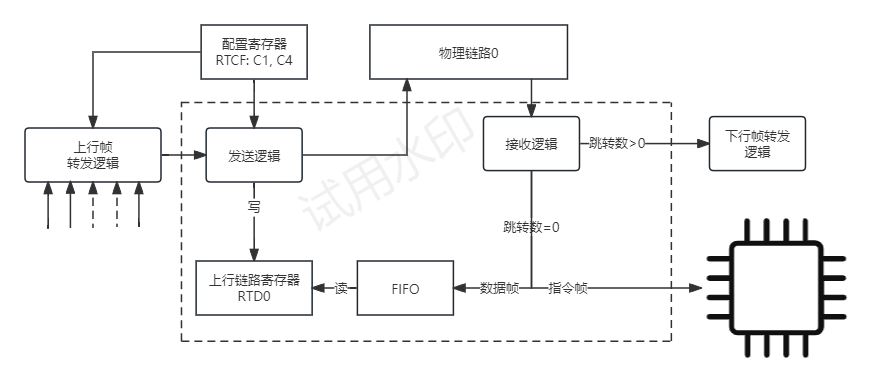
\includegraphics[width=1.0\linewidth]{rtmq/rtmq_link_up}
% \end{figure}


% 下级节点x收发逻辑模块内部结构如图\ref{fig:rtmq_link_down}所示,它包含发送逻辑x模块、接收逻辑x模块和先进先出队列模块FIFOx三个子模块。发送逻辑x模块用于构建下行帧,并交由物理链路x模块发送;接收逻辑x模块用于接收来自下级节点x的上行帧,并根据其跳转数和帧类型对其进行进一步处理;先进先出队列模块FIFOx:用于按顺序存储来自下级节点x且跳转数为0的上行数据帧的载荷。


% \begin{figure}
%     \centering
%     \caption[下级节点x收发逻辑模块内部结构图]{下级节点x收发逻辑模块内部结构图\label{fig:rtmq_link_down}}
%     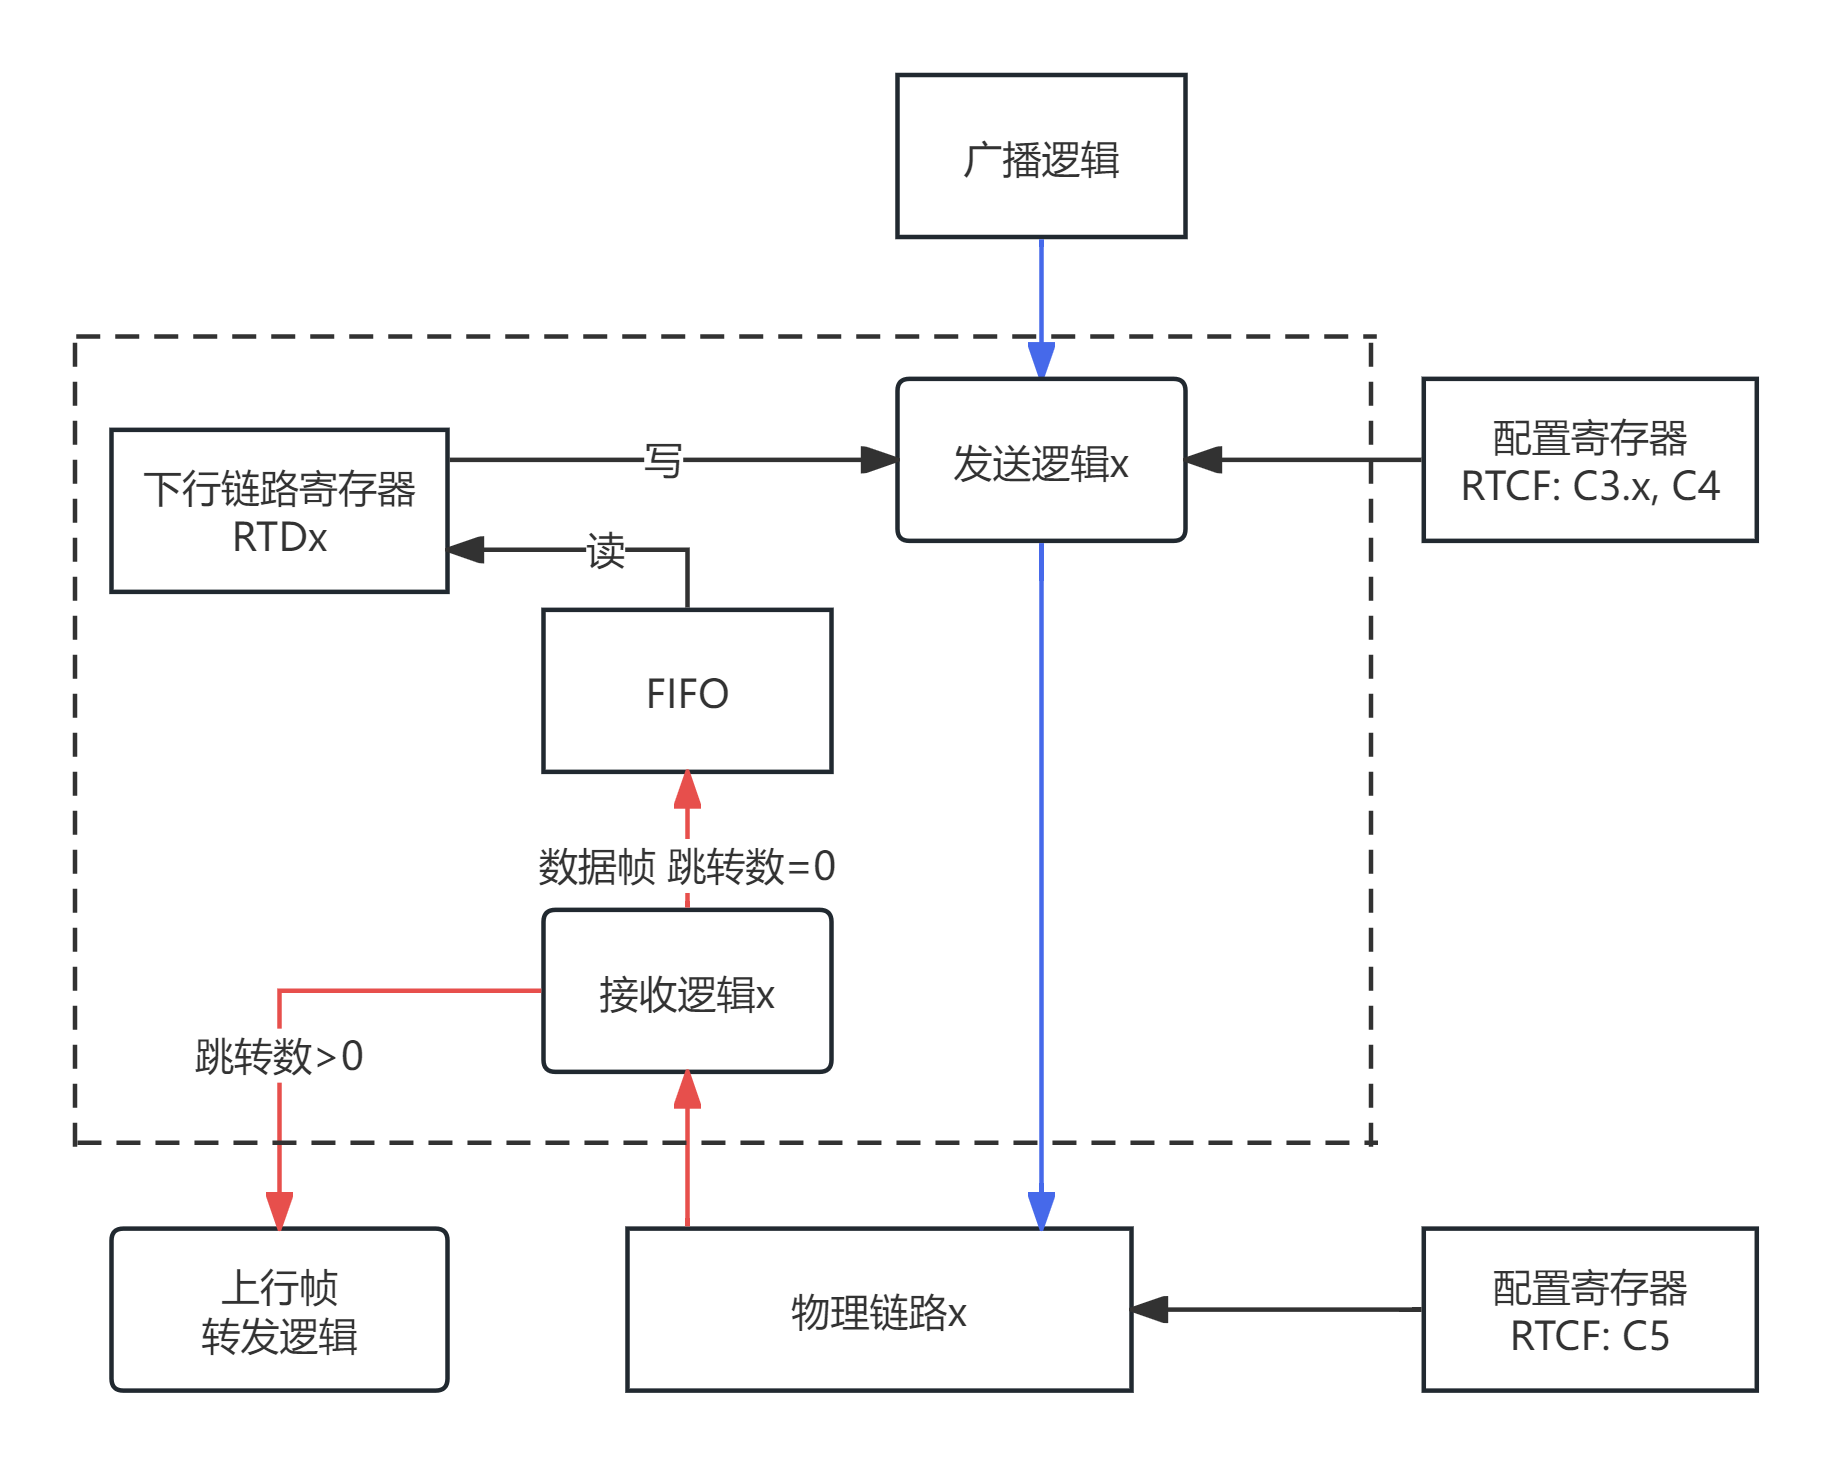
\includegraphics[width=1.0\linewidth]{rtmq/rtmq_link_down}
% \end{figure}




% 广播逻辑模块内部结构如图\ref{fig:rtmq_link_broadcast}所示,它包含下行帧转发逻辑模块和上行帧转发逻辑模块两个子模块。当RTCF配置C2为P2.0(来自RTBC)时,向该模块RTBC写入数据将构建下行帧,并同时分发给所有下级节点收发逻辑模块进一步处理;当RTCF配置C2为P2.1(转发来自上级节点的下行帧)时,则将来自上级节点的下行帧同时交由所有下级节点收发逻辑模块进一步处理。

% \begin{figure}
%     \centering
%     \caption[广播逻辑模块内部结构图]{广播逻辑模块内部结构图\label{fig:rtmq_link_broadcast}}
%     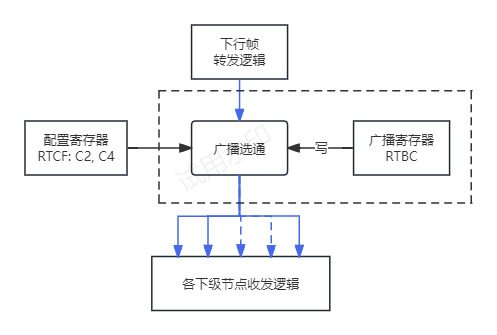
\includegraphics[width=1.0\linewidth]{rtmq/rtmq_link_broadcast}
% \end{figure}





\subsection[实时通信链路系统实施例]{实时通信链路系统实施例}


基于上述介绍的RTMQ节点间实时通信的链路系统,本节给出其在一个由7个节点组成的实验系统中具体的实施案例。该实验测控系统由13个RTMQ节点构成,包含1个直接与控制整个系统上位机连接的根节点。该根节点具有2个下级节点,分别记为节点1、节点2;其中节点1包含1个下级节点,节点1.1;节点2包含3个下级节点,节点2.1、节点2.2,、节点2.3。所有节点之间通过速率为10Mbps、包含1个停止位和8个数据位的UART链路连接。
% 通信帧的魔术字位宽为4位,取值0xA,跳转数的位宽为3位,载荷位宽为32位,从而帧的总位宽为40位。

基于此系统,下面给出一个跨节点实时反馈的实施案例。假设节点2需要根据节点1采集到的数据决定后续执行流程,若小于阈值,则执行函数a,否则执行函数b。

\begin{table}
    \centering
    \caption[跨节点实时反馈的案例实施步骤]{跨节点实时反馈的案例实施步骤\label{tb:rtmq_notes_synchronize}}
    \begin{tabular}{C{3cm}|C{11cm}}
        \toprule
        节点 & 节点步骤操作 \\
        \midrule
        节点1步骤 & 操作\\
        \hline
        1.1 & 采集数据\\
        1.2 & RTCF的配置C1设为选项P1.0\\
        1.3 & RTCF的配置C4设为:帧类型:数据帧,跳转数:0\\
        1.4 & 向RTD0写入采集到的数据\\
        \midrule
        根节点步骤 & 操作 \\
        \hline
        R.1 & 当FIFO1非空时,从RTD1读取节点1发来的数据\\
        R.2 & RTCF的配置C3.2设为选项P3.2.0\\
        R.3 & RTCF的配置C4设为:帧类型:指令帧,跳转数:0\\
        R.4 & 向RTD2写入指令,若读取到的数据小于阈值,指令为调用函数a,否则指令为调用函数b\\
        \midrule
        节点2步骤 & 操作 \\
        \hline
        2.1 & 在收到来自根节点的指令前处于挂起状态 \\
        \bottomrule
    \end{tabular}
\end{table}

如表\ref{tb:rtmq_notes_synchronize}所示,节点1按顺序执行以下步骤:
步骤1.1:采集数据;
步骤1.2:RTCF的配置C1设为选项P1.0;
步骤1.3:RTCF的配置C4设为:帧类型:数据帧,跳转数:0;
步骤1.4:向RTD0写入采集到的数据;
根节点按顺序执行以下步骤:
步骤R.1:当FIFO1非空时,从RTD1读取节点1发来的数据;
步骤R.2:RTCF的配置C3.2设为选项P3.2.0;
步骤R.3:RTCF的配置C4设为:帧类型:指令帧,跳转数:0;
步骤R.4:向RTD2写入指令,若读取到的数据小于阈值,指令为“调用函数a”,否则指令为“调用函数b”;
节点2在收到来自根节点的指令前,处于挂起状态。


前述实施案例的原理为UART链路传递一个字节需要传递1个起始位、8个数据位和1个停止位,合计10个比特,因此传递1个通信帧的时间开销为精确的5us,解决方案A中的跨节点反馈操作的通信开销为10us。其优势在于各节点所执行的指令序列没有任何不确定性,整个反馈控制的总开销可以精确到单个时钟周期,符合实时控制的要求。


基于此系统,下面给出同步多个下级节点的执行时序的实施案例。假设节点2的3个下级节点需要严格同时开始执行某功能,比如同时对三个离子进行态初始化操作。

\begin{table}
    \centering
    \caption[多节点同步的案例实施步骤]{多节点同步的案例实施步骤\label{tb:rtmq_synchronize_start}}
    \begin{tabular}{C{3cm}|C{11cm}}
        \toprule
        节点 & 节点步骤操作\\
        \midrule
        节点2步骤 & 操作\\
        \hline
        2.1 & RTCF的配置C2设为选项P2.0\\
        2.2 & RTCF的配置C3.1设为选项P3.1.1,配置C3.2设为选项P3.2.1,配置C3.3设为选项P3.3.1\\
        2.3 & RTCF的配置C4设为:帧类型:指令帧,跳转数:0\\
        2.4 & 向RTBC写入解除挂起状态指令\\
        \midrule
        节点2.1步骤 & 操作 \\
        \hline
        2.1 & 在收到解除挂起状态指令前处于挂起状态 \\
        \midrule
        节点2.2步骤 & 操作 \\
        \hline
        2.2 & 在收到解除挂起状态指令前处于挂起状态 \\
        \midrule
        节点2.3步骤 & 操作 \\
        \hline
        2.3 & 在收到解除挂起状态指令前处于挂起状态 \\
        \bottomrule
    \end{tabular}
\end{table}

如表\ref{tb:rtmq_synchronize_start}所示,节点2按顺序执行以下步骤:
步骤2.1:RTCF的配置C2设为选项P2.0;
步骤2.2:RTCF的配置C3.1设为选项P3.1.1,配置C3.2设为选项P3.2.1,配置C3.3设为选项P3.3.1;
步骤2.3:RTCF的配置C4设为:帧类型:指令帧,跳转数:0;
步骤2.4:向RTBC写入“解除挂起状态”指令;
节点2.1、节点2.2和节点2.3在收到指令前处于挂起状态;

前述实施案例的原理为节点间传递1帧的开销为精确的5us,利用广播逻辑模块,可以使得节点2的物理链路1-3模块同时进入发送状态,从而节点2.1、节点2.2和节点2.3同时收到“解除挂起状态”的指令,同时开始执行后续任务。其优势在于可以精确控制不同节点严格同步执行各种任务,且利用广播模块可以轻松拓展到几百上千个节点数,可以很好地满足该同步触发类应用场景的要求。



基于此系统,下面给出对任意节点进行非实时配置和检查的实施案例。假设上位机在实验开始前需要对节点2.3进行配置和检查。


\begin{table}
    \centering
    \caption[对任意节点配置的案例实施步骤]{对任意节点配置的案例实施步骤\label{tb:rtmq_notes_config}}
    \begin{tabular}{C{3cm}|C{11cm}}
        \toprule
        节点 & 节点步骤操作 \\
        \midrule
        节点2步骤 & 操作\\
        \hline
        2.1 & RTCF的配置C1设为选项P1.3\\
        2.2 & RTCF的配置C2设为选项P2.1\\
        2.3 & RTCF的配置C3.3设为选项P3.3.1\\
        \midrule
        根节点步骤 & 操作 \\
        \hline
        R.1 & RTCF的配置C3.3设为选项P3.3.0\\
        R.2 & RTCF的配置C4设为:帧类型:指令帧,跳转数:1\\
        R.3 & 将所需的配置指令按顺序逐条写入RTD3\\
        R.4 & 若FIFO3非空,则从RTD3逐个读取数据并转发给上位机,直到FIFO3为空\\
        \midrule
        节点2.3步骤 & 操作 \\
        \hline
        2.3.1 & 收到指令前处于挂起状态,其RTCF的各项配置可通过根节点发送的指令帧进行设置 \\
        \bottomrule
    \end{tabular}
\end{table}

如表\ref{tb:rtmq_notes_config}所示,节点2按顺序执行以下步骤:
步骤2.1:RTCF的配置C1设为选项P1.3;
步骤2.2:RTCF的配置C2设为选项P2.1;
步骤2.3:RTCF的配置C3.3设为选项P3.3.1;
根节点按顺序执行以下步骤:
步骤R.1:RTCF的配置C3.3设为选项P3.3.0;
步骤R.2:RTCF的配置C4设为:帧类型:指令帧,跳转数:1;
步骤R.3:将所需的配置指令按顺序逐条写入RTD3;
步骤R.4:若FIFO3非空,则从RTD3逐个读取数据并转发给上位机,直到FIFO3为空;
节点2.3在收到指令前处于挂起状态,其RTCF的各项配置可通过根节点发送的指令帧进行设置,若需要节点2.3返回数据,则RTCF的正确配置为:
配置C1设为选项P1.0;
配置C4设为:帧类型:数据帧,跳转数:1;
而后根节点通过向其发送指令帧,令其将所需数据写入RTD0即可。

前述实施案例的原理为将节点2的RTCF配置为一种“透明转发”状态,即直接向节点2.3转发来自根节点的下行帧,并且直接向根节点转发来自节点2.3的上行帧。如此,对于系统中的任一节点,只需将根节点到该目标节点之间途经的所有节点都设置成这种“透明转发”状态,即可直接对该目标节点进行控制和访问。其优势在于这些配置都在实验前进行,因而不会影响实际实验任务的执行。
当需要对整个系统中所有节点进行配置时,可以先逐个配置所有的叶节点,再逐个配置其下级节点已经全部完成配置的中间结点,以此类推,直到最后配置根节点,如此,可以保证系统中所有的节点在配置完成后,状态不会受到额外的干扰。


% \section[RTMQ的重要功能外设及其FPGA实现]{RTMQ的重要功能外设及其FPGA实现}
% % ============================================================================
% % ============================================================================
% % =======================   RTMQ Peripheral    ===============================
% % ============================================================================
% % ============================================================================
% RTMQ量子测控系统的整体构成不仅需要一个专为实时可拓展量子计算设计的微处理器核心,还需要其它功能性模块的参与。因此与RTMQ架构相配套的功能性模块的设计开发必不可少,其中比较重要的有通用寄存器模块、用于节点之间及与上位机通信的UART或SPI等通信模块、用于外部芯片的管理模块、用于实验系统反馈控制的高速通用数字PID模块和用于过滤噪声提高信号质量的高速通用数字IIR滤波器模块等,这些模块的设计和基于FPGA的实现将在本节接下来的几小节中进行介绍。

% % \subsection[RTMQ的重要系统外设及其FPGA实现]{RTMQ的重要系统外设及其FPGA实现}
% % % ============================================================================
% % % =======================RTMQ System Peripheral===============================
% % % ============================================================================

% % \subsubsection[指令缓存、数据缓存、节点信息只读储存器及其FPGA实现]{指令缓存、数据缓存、节点信息只读储存器及其FPGA实现}

% % \subsubsection[地址栈模块及其FPGA实现]{地址栈模块及其FPGA实现}

% % \subsubsection[数据栈模块及其FPGA实现]{数据栈模块及其FPGA实现}

% % \subsubsection[内存模块及其FPGA实现]{内存模块及其FPGA实现}




% % \subsection[RTMQ重要功能外设及其FPGA实现]{RTMQ重要功能外设及其FPGA实现}
% % ============================================================================
% % ======================RTMQ External Peripheral==============================
% % ============================================================================

% \subsection[通用寄存器模块及其FPGA实现]{通用寄存器模块及其FPGA实现}
% % =======================     通用寄存器模块    ===============================
% 通用寄存器(General-Purpose Registers)是微处理器的一个重要功能外设,用于存储和操作微处理器中的数据。它可以用于临时存储指令和数据,以支持计算、逻辑操作和数据传输等操作,是微处理器与其它功能性外设联系的纽带。RTMQ核心的算数和逻辑运算操作、内部数据的传递和结果的储存、地址计算等都需要借助通用寄存器来实现。除此之外,通用寄存器也可以提供接口给其它功能性外设对其进行参数传递和读取,提高参数传递的速度和灵活性。接下来将介绍RTMQ系统中的通用寄存器模块及其FPGA实现结果。

% 通用寄存器的功能是根据微处理器请求的寄存器地址对相应的寄存器进行高速的读或写操作。RTMQ中的通用寄存器接收来自算术逻辑单元的结果alu\_out,给出寄存器的数据输出reg\_out和副作用触发信号f\_trg。其中alu\_out的输出结构alu\_out为:\{alu\_res, alu\_msk, alu\_rda, alu\_r0a, alu\_r1a, imm\_res, imm\_rda, imm\_seg\},信号具体含义如第\ref{section:rtmq_core_alu}节所述;reg\_out是寄存器的数据输出;f\_trg是寄存器的副作用触发信号,可以用来为寄存器的特定应用定义一些额外的功能。RTMQ\_AcsFlg模块的功能是根据alu\_out中寄存器地址位的值给出对该地址的寄存器的读写信号,

% 如图\ref{fig:rtmq_universal_register}所示,如表\ref{tb:rtmq_universal_register}所示。\textcolor{green}{具体内容描述待补充。}

% \begin{table}
%     \centering
%     \caption[RTMQ系统外设通用寄存器模块端口定义]{RTMQ系统外设通用寄存器模块端口定义\label{tb:rtmq_universal_register}}    
%     \begin{tabular}{L{2.5cm}L{4cm}|L{2.5cm}L{4cm}}
%         \toprule
%         \multicolumn{2}{c|}{Input} & \multicolumn{2}{c}{Output} \\
%         \midrule
%         Port & Define & Port & Define\\
%         \hline
%         alu\_out[128:0] & 算术逻辑单元结果  & f\_trg & 副作用触发信号 \\
%         clk             & 系统时钟          & reg\_out[31:0] & 寄存器数据输出 \\
%         \bottomrule
%     \end{tabular}
% \end{table}


% \begin{figure}
%     \centering
%     \caption[RTMQ用寄存器模块的FPGA实现结构图]{RTMQ用寄存器模块的FPGA实现结构图\label{fig:rtmq_universal_register}}
%     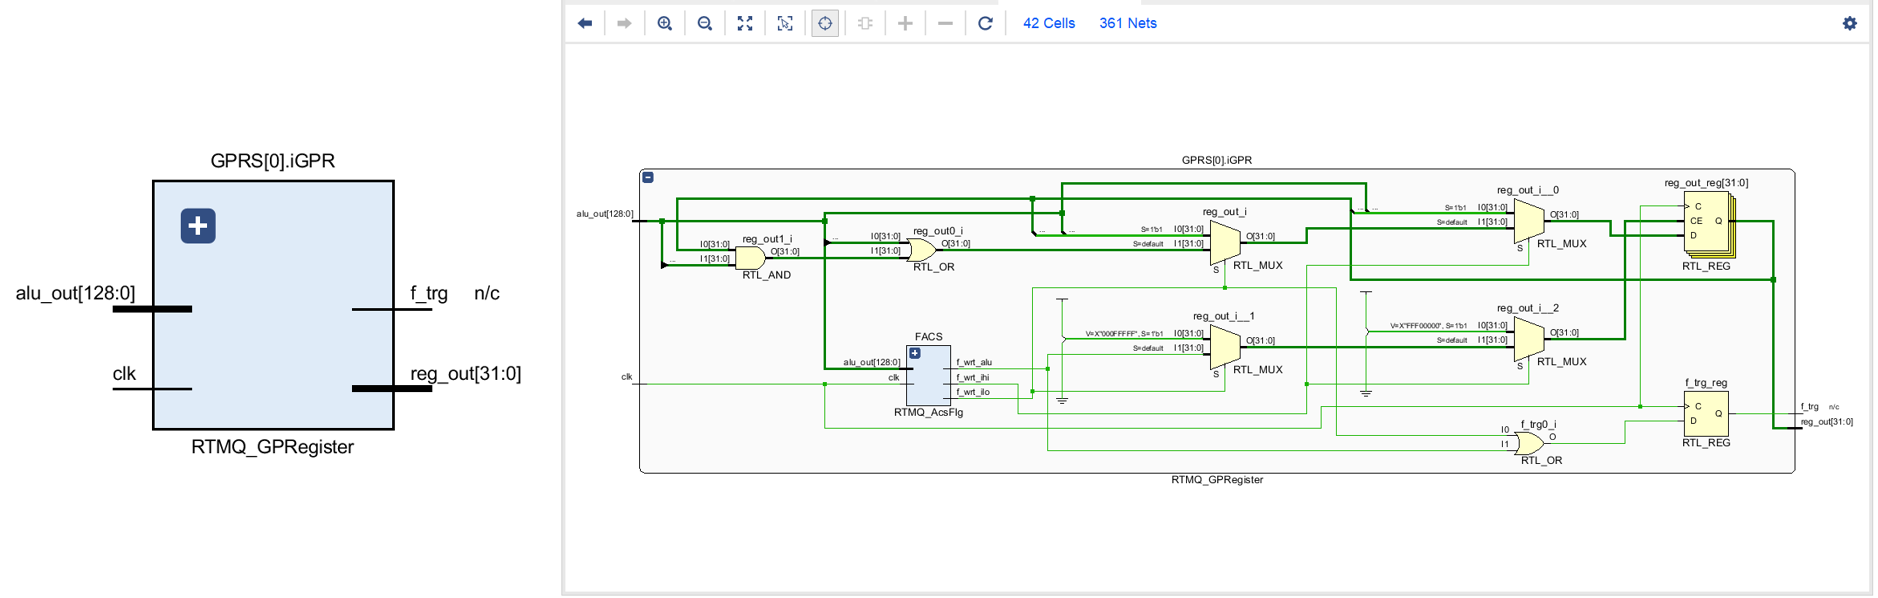
\includegraphics[width=1.0\linewidth]{rtmq/rtmq_universal_register}
% \end{figure}



% \subsection[UART模块及其FPGA实现]{UART模块及其FPGA实现}
% % =======================       UART模块       ===============================
% 通信模块是RTMQ系统与上位机以及RTMQ系统节点之间相互传递信息的重要模块,其中UART通信模块在整个RTMQ系统中有着十分广泛的应用。UART模块即通用异步收发器(Universal Asynchronous Receiver/Transmitter),特点是通信线路简单,适用于远距离通信,但传输速度慢。因此该种通信方式主要应用于RTMQ系统节点与上位之间的通信以及RTMQ节点之间同步信息传递。接下来将介绍RTMQ系统中的UART模块及其FPGA实现结果。

% % \subsubsection[UART模块原理]{UART模块原理}
% UART是一种串行、异步、全双工的通信协议,它的数据通信格式如表\ref{tb:rtmq_uart_data}所示。根据UART协议,初始时总线处于空闲状态,即信号线为高电平“1”(空闲位);每次传输开始时对方先发出一个低电平“0”(起始位);起始位之后就是数据位,可以是6、7、8、9位等等,先发送低位再发送高位,使用低电平表示‘0’高电平表示‘0’(有效数据位);根据事先规定,数据位加上这一位后,使得“1”的位数应为偶数(偶校验)或奇数(奇校验),以此来校验数据传送的正确性(奇偶校验位);一次字符数据传输结束后给出若干位高电平指示本字节传输结束,可以是1位、1.5位、2位等(停止位)。

% \begin{table}
%     \centering
%     \caption[UART数据通信格式]{UART数据通信格式。起始位之前和停止位之后是空闲位;最低位LSB到最高位MSB之间为有效数据位;奇偶校验位在MSB之后。\label{tb:rtmq_uart_data}}    
%     \begin{tabular}{C{0.9cm}|C{0.85cm}C{0.4cm}C{0.4cm}C{0.4cm}C{0.4cm}C{0.4cm}C{0.4cm}C{0.4cm}C{0.4cm}C{0.85cm}|C{0.9cm}C{0.9cm}|C{0.9cm}}
%         % \begin{tabular}{cccccccccccccc}
%         \toprule
%         &\multicolumn{12}{c}{第n个字节数据流}& \\
%         \midrule
%         1 & 0 & X & X & X & X & X & X & X & X & X & X & 1 & 1 \\
%         \hline
%         空闲位 & 起始位 & LSB & & & & & & & & MSB & 奇偶校验位 & 停止位 & 空闲位 \\ 
%         % & \multirow{10}{*}{有效数据位} &  &  & \\
%         \bottomrule
%     \end{tabular}
% \end{table}

% 通过UART通信协议的理解,UART模块的组成主要有两部分:发送模块和接收模块。另外,该模块的开发也要结合RTMQ核心模块的处理方式,以使得RTMQ核心能够直接通过其通用寄存器对UART进行控制。模块的实现结构如图\ref{fig:rtmq_uart_structure}所示,主要用到的模块有寄存器、RTMQ通用寄存器模块、UART发送模块、UART接收模块等,另外对接收的信息进行了逻辑处理以保证输出始终为可供RTMQ核心使用的合法数据。接口主要有RTMQ算术逻辑单元输入、UART接收输入、配置指令输出、配置指令覆盖标志、发送信号、发送结束标志等。

% \begin{figure}
%     \centering
%     \caption[RTMQ功能外设UART模块的FPGA实现结构图]{RTMQ功能外设UART模块的FPGA实现结构图\label{fig:rtmq_uart_structure}}
%     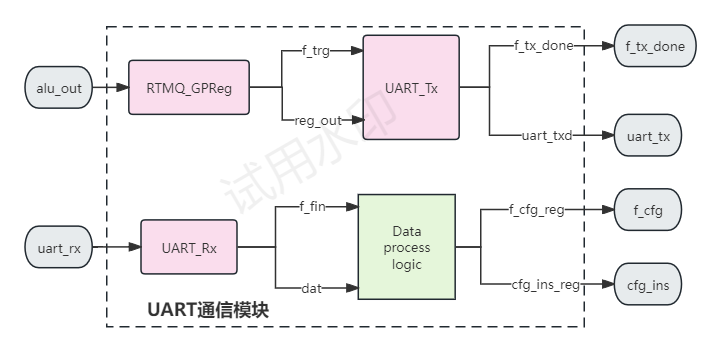
\includegraphics[width=1.0\linewidth]{rtmq/rtmq_uart_structure}
% \end{figure}

% % \subsubsection[UART模块的FPGA实现]{UART模块的FPGA实现}

% UART通信模块在Vivado中的FPGA实现结果如图\ref{fig:rtmq_uart}所示,其具体的接口定义如表\ref{tb:rtmq_uart}所示。
% % \textcolor{green}{具体内容描述待补充。}


% \begin{table}
%     \centering
%     \caption[RTMQ系统外设UART模块端口定义]{RTMQ系统外设UART模块端口定义\label{tb:rtmq_uart}}    
%     \begin{tabular}{L{2.5cm}L{4cm}|L{2.5cm}L{4cm}}
%         \toprule
%         \multicolumn{2}{c|}{Input} & \multicolumn{2}{c}{Output} \\
%         \midrule
%         Port & Define & Port & Define\\
%         \hline
%         alu\_out[128:0] & 算术逻辑单元结果  & cfg\_ins[31:0] & 模块配置指令 \\
%         clk             & 系统时钟          & f\_cfg & 配置指令覆盖标志 \\
%         uart\_rx        & UART接受信号Rx    & f\_tx\_done & 发送信号结束标志 \\
%         &               & uart\_tx          & UART发送信号Tx\\
%         \bottomrule
%     \end{tabular}
% \end{table}

% \begin{figure}
%     \centering
%     \caption[RTMQ功能外设UART模块的FPGA实现结构图]{RTMQ功能外设UART模块的FPGA实现结构图(Vivado)。\label{fig:rtmq_uart}}
%     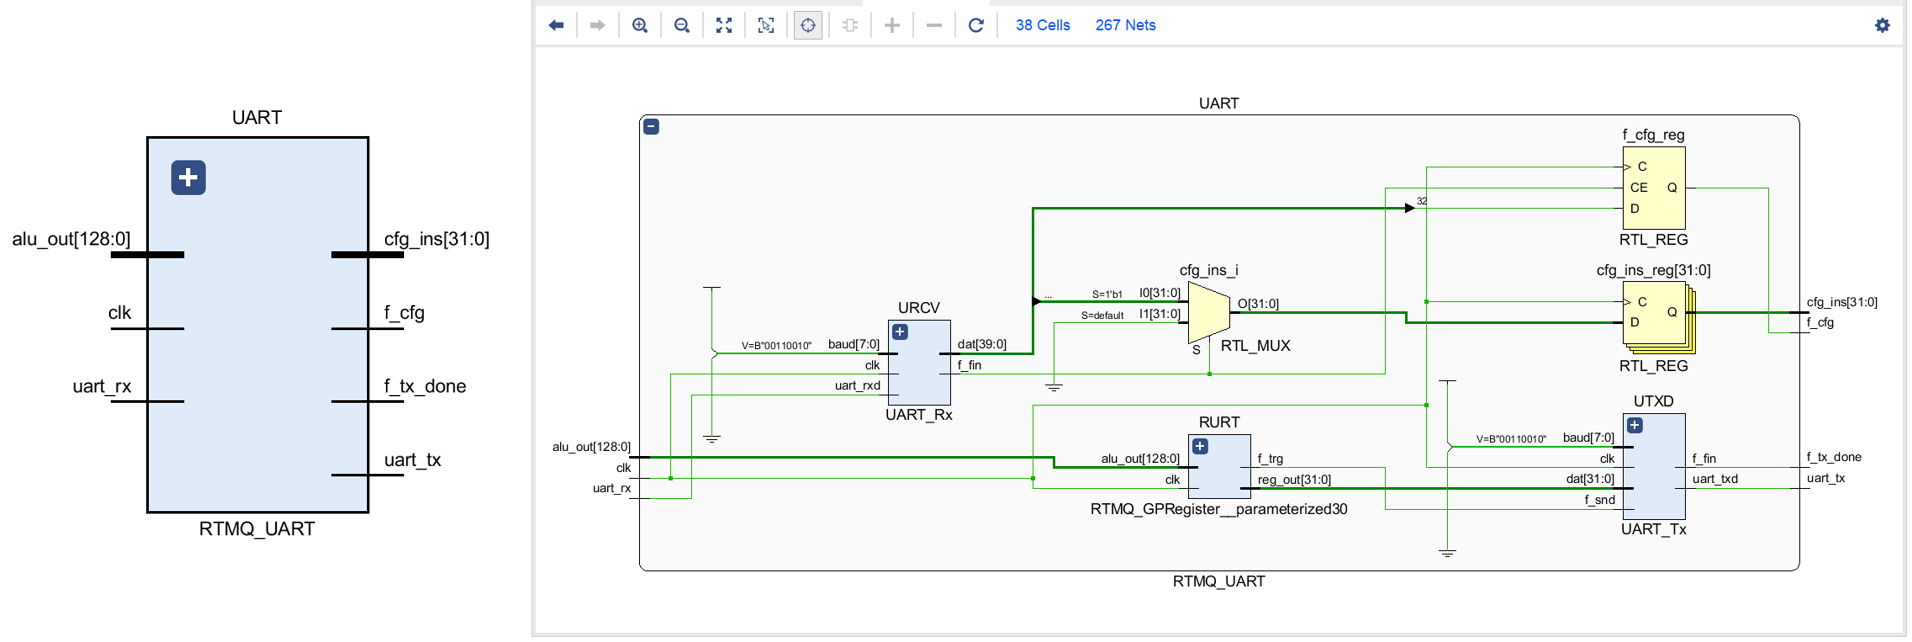
\includegraphics[width=1.0\linewidth]{rtmq/rtmq_uart}
% \end{figure}




% \subsection[SPIMaster模块及其FPGA实现]{SPIMaster模块及其FPGA实现}
% % =======================        SPI模块       ===============================

% RTMQ系统中不仅涉及与上位机和不同RTMQ节点间相互的通信,还需要与一些如板上的其它功能芯片进行高速通信。在高速通信的场景下UART通信协议的应用很受限,因此需要一种可以支持高速通信的协议来满足需求——SPI(串行外围设备接口,Serial Perripheral Interface)。SPI是一种高速、全双工、同步的通信总线,它常用于EEPROM、Flash、实时时钟(RTC)、数模转换器(ADC)、数字信号处理器(DSP) 以及数字信号解码器之间。RTMQ系统的微处理器即采用SPI进行外部功能拓展设备的管理,如与板上集成的AD9910芯片间的通信等。

% SPI通信模块在Vivado中的FPGA实现如图\ref{fig:rtmq_spi}所示,其具体的接口定义如表\ref{tb:rtmq_spi}所示。

% \textcolor{green}{具体内容描述待补充。}


% \begin{table}
%     \centering
%     \caption[RTMQ系统外设SPIMaster模块端口定义]{RTMQ系统外设SPIMaster模块端口定义\label{tb:rtmq_spi}}    
%     \begin{tabular}{L{2.5cm}L{4cm}|L{2.5cm}L{4cm}}
%         \toprule
%         \multicolumn{2}{c|}{Input} & \multicolumn{2}{c}{Output} \\
%         \midrule
%         Port & Define & Port & Define\\
%         \hline
%         alu\_out[128:0] & 算术逻辑单元结果 & csb &  \\
%         clk & 系统时钟 & f\_spi\_done & SPI Rx/Tx结束标志 \\
%         miso & 主收从发信号 & mosi & 主发从收信号 \\
%         & & reg\_sctl[31:0] & \\
%         & & reg\_sdat[31:0] & \\
%         & & sclk & 主设备产生的时钟信号 \\
%         & & slv\_adr[2:0] & 目标从设备地址\\

%         \bottomrule
%     \end{tabular}
% \end{table}

% \begin{figure}
%     \centering
%     \caption[RTMQ功能外设SPIMaster模块的FPGA实现结构图]{RTMQ功能外设SPIMaster模块的FPGA实现结构图\label{fig:rtmq_spi}}
%     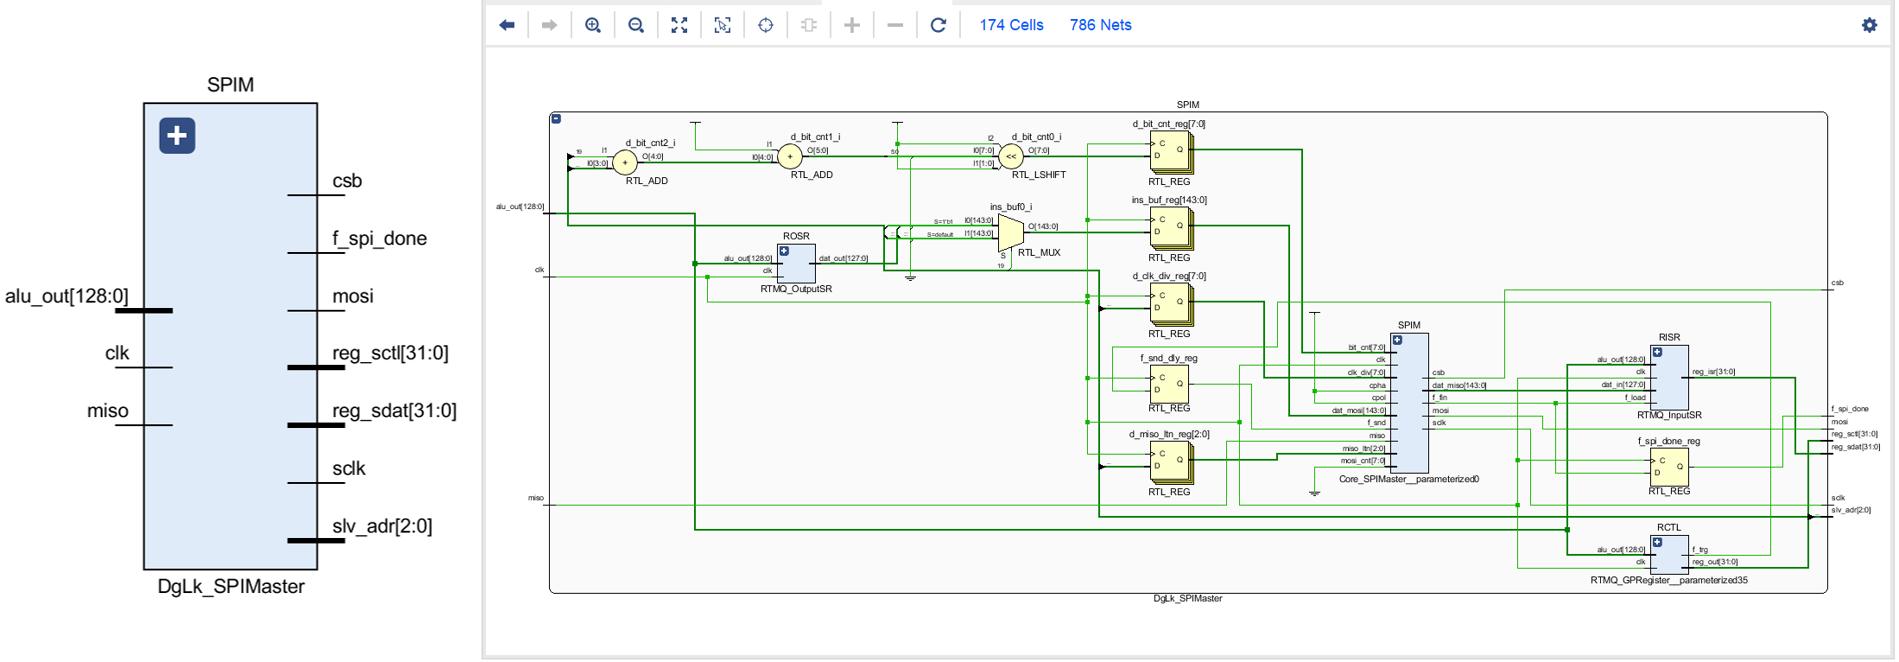
\includegraphics[width=1.0\linewidth]{rtmq/rtmq_spi}
% \end{figure}



% \subsection[AD9910芯片管理模块及其FPGA实现]{AD9910芯片管理模块及其FPGA实现}
% % =======================    AD9910管理模块     ===============================


% 如图\ref{fig:rtmq_ad9910}所示,如表\ref{tb:rtmq_ad9910}所示。\textcolor{green}{具体内容描述待补充。}


% \begin{table}
%     \centering
%     \caption[RTMQ系统外设AD9910芯片管理模块端口定义]{RTMQ系统外设AD9910芯片管理模块端口定义\label{tb:rtmq_ad9910}}    
%     \begin{tabular}{L{2.5cm}L{4cm}|L{2.5cm}L{4cm}}
%         \toprule
%         \multicolumn{2}{c|}{Input} & \multicolumn{2}{c}{Output} \\
%         \midrule
%         Port & Define & Port & Define\\
%         \hline
%         alu\_out[128:0] & 算术逻辑单元结果  & io\_rst & 输入输出充值信号 \\
%         cdds[12:0]      & DDS控制信号       & io\_upd & 输入输出更新信号 \\
%         clk             & 系统时钟          & m\_rst & 主机重置信号 \\
%         pda\_clk        & PD时钟            & pdat[15:0] & 并行数据 \\
%         syn\_clk        & 同步时钟          & pf[1:0] & 并行数据目标 \\
%                         &                   & reg\_cmn[31:0] & 时钟相位检测\\
%                         &                   & tx\_en & 发送使能信号\\
%         \bottomrule
%     \end{tabular}
% \end{table}


% \begin{figure}
%     \centering
%     \caption[RTMQ功能外设UART模块的FPGA实现结构图]{RTMQ功能外设UART模块的FPGA实现结构图\label{fig:rtmq_ad9910}}
%     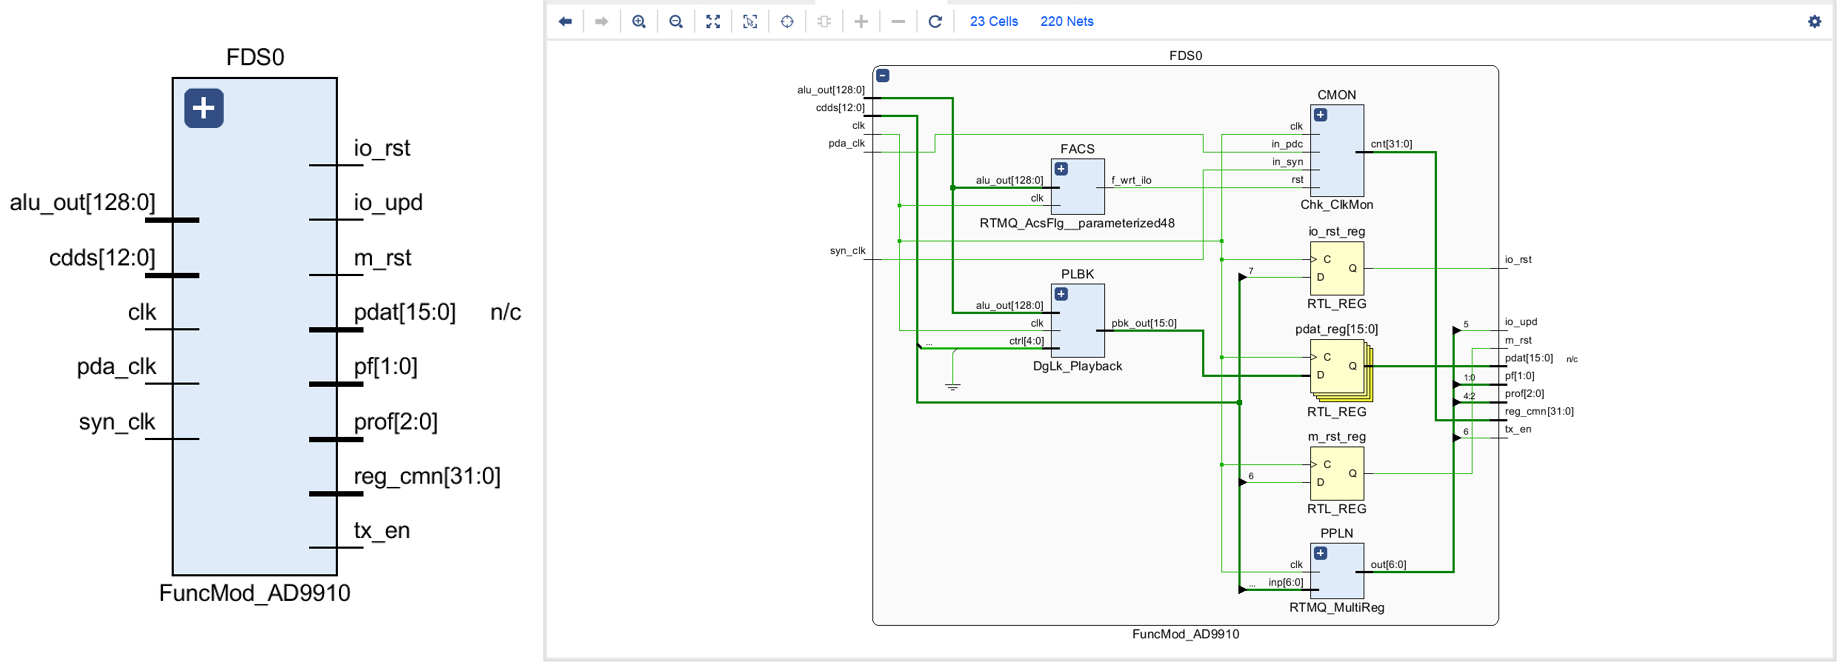
\includegraphics[width=1.0\linewidth]{rtmq/rtmq_ad9910}
% \end{figure}




% \subsection[ADC芯片管理模块及其FPGA实现]{ADC芯片管理模块及其FPGA实现}
% % =======================      ADC管理模块      ===============================


% 如图\ref{fig:rtmq_adc}所示,如表\ref{tb:rtmq_adc}所示。\textcolor{green}{具体内容描述待补充。}


% \begin{table}
%     \centering
%     \caption[RTMQ系统外设AD9910芯片管理模块端口定义]{RTMQ系统外设AD9910芯片管理模块端口定义\label{tb:rtmq_adc}}    
%     \begin{tabular}{L{2.5cm}L{4cm}|L{2.5cm}L{4cm}}
%         \toprule
%         \multicolumn{2}{c|}{Input} & \multicolumn{2}{c}{Output} \\
%         \midrule
%         Port & Define & Port & Define\\
%         \hline
%         adc\_in[15:0]   & ADC采样数据   & reg\_aio[15:0] & ADC输出数据 \\
%         adc\_smp        & ADC采样时钟   &  &  \\
%         clk             & 系统时钟      &  &  \\
%         \bottomrule
%     \end{tabular}
% \end{table}




% \begin{figure}
%     \centering
%     \caption[RTMQ功能外设ADC模块的FPGA实现结构图]{RTMQ功能外设ADC模块的FPGA实现结构图\label{fig:rtmq_adc}}
%     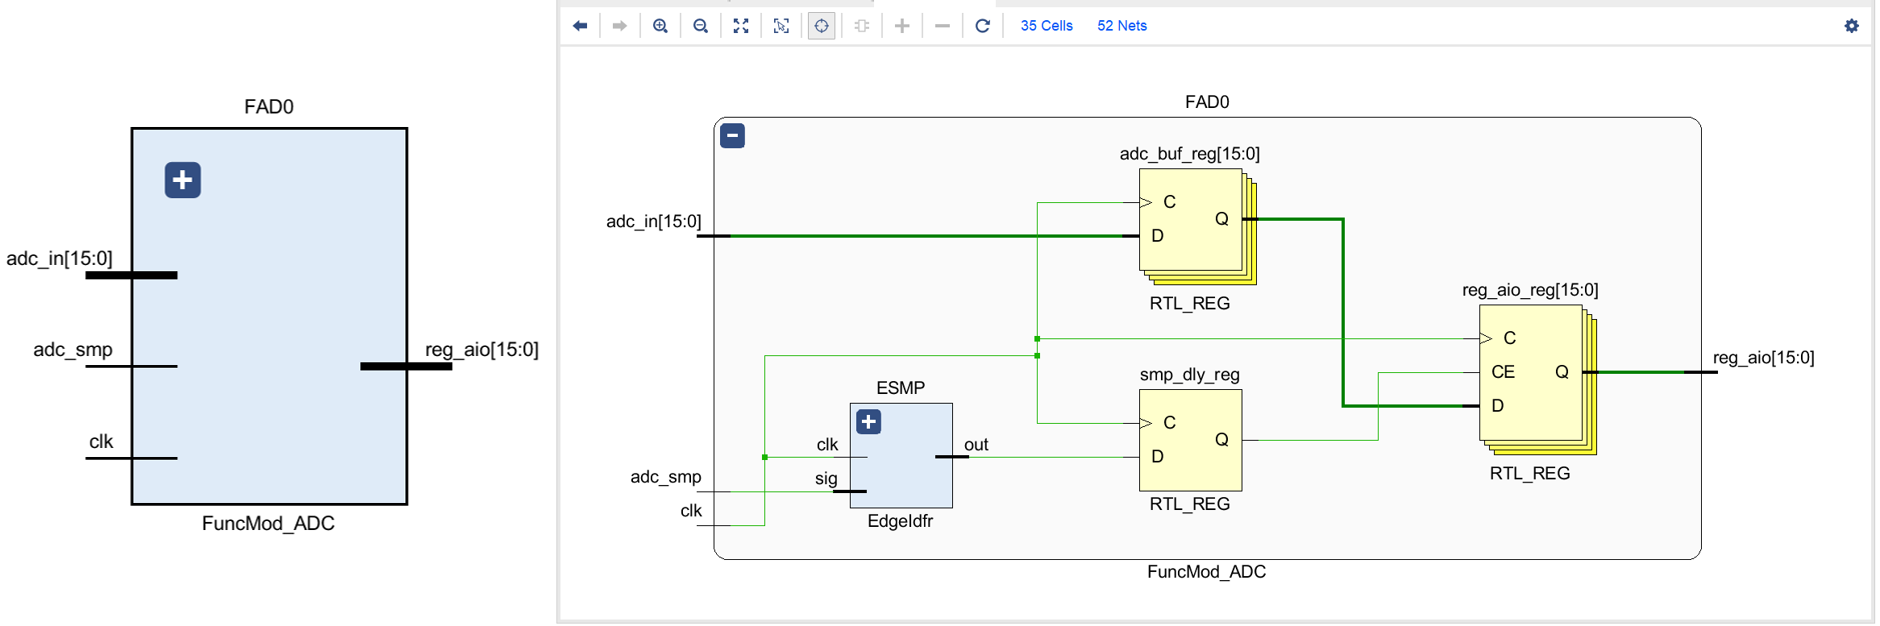
\includegraphics[width=1.0\linewidth]{rtmq/rtmq_adc}
% \end{figure}

% % \subsubsection[随机数发生器模块及其FPGA实现]{随机数发生器模块及其FPGA实现}



% \subsection[高速通用数字PID及其FPGA实现]{高速通用数字PID及其FPGA实现\label{section:digital_pid}}
% % ============================================================================
% % =======================      高速数字PID      ===============================
% % ============================================================================


% 当前量子计算系统中大量采用PID控制器进行诸如激光功率稳定、激光相位稳定、激光拍频锁定等等控制系统的构建,常用的器件有如LB1005模拟伺服控制器。这类模拟控制器的确定在于稳定性较差且价格昂贵,此外它的集成度也比较差,往往需要占用较大的实验平台面积。除此之外这类模拟PID控制器往往采用机械旋钮进行参数调节,不利于进行实验系统的集成化和自动化。与之相比较,使用融合了高速通用数字PID的RTMQ测控系统可以同时完成对实验序列的操控和对设备关键参数的伺服控制。除此之外,采用也对系统完成了集成化和数字化,提高了系统的稳定性和易用性。

% \subsubsection[数字PID]{数字PID}
% 数字PID控制器是一种常用的自动控制算法,用于实现对系统的闭环控制。PID控制器通过对系统的误差进行比例(Proportional)、积分(Integral)和微分(Derivative)计算,生成控制信号来调整系统的输出,以达到期望的控制效果。在量子测控系统中很多地方都需要用到闭环控制,比如激光的功率稳定、激光的波长稳定、离子阱频率稳定等。相对于模拟PID控制器,数字PID控制器具有结构简单、易于实现、控制灵活、工作稳定等优点,是RTMQ系统中的重要组成部分。

% PID 控制器的数学表达式可以表示为:
% \begin{align}
%     u(t)= K_p e(t) + K_i \int_{0}^{t} e(\tau) d\tau + K_d \frac{d e(t)}{dt}
% \end{align}

% 其中,$u(t)$是控制器的输出,$e(t)$是系统的误差,$K_p$、$K_i$和$K_d$分别是比例系数、积分系数和微分系数。
 
% PID控制器的实现可以分为模拟PID和数字PID两种方式。模拟PID是通过模拟电路实现的,而数字PID是通过数字计算实现的。数字PID控制器通常使用微处理器或计算机来实现,其基本结构包括采样、计算和输出三个部分。数字 PID 控制器的实现步骤如下:
% \begin{itemize}
%     \item 采样:对系统的输入和输出进行采样,获取当前时刻的误差值e(t);
%     \item 计算:根据采样得到的误差值,按照 PID 控制器的数学表达式计算控制信号u(t);
%     \item 输出:将计算得到的控制信号输出到执行机构,调整系统的输出;
% \end{itemize}

% 在数字PID控制器的实现中,需要对积分和微分操作进行离散化处理。常用的离散化方法有矩形法和梯形法。矩形法将积分区间划分为若干个相等的子区间,每个子区间的积分值近似为矩形的面积;梯形法将积分区间划分为若干个相等的子区间,每个子区间的积分值近似为梯形的面积。这一步骤在嵌入式系统中通常使用模拟数字转换(ADC)芯片来完成。

% \subsubsection[数字PID的增量表达式]{数字PID的增量表达式}
% 硬件资源在FPGA中是十分宝贵的资源,而乘法器这样的器件往往会占用大量的硬件资源。因此在满足时序要求的情况下我们希望能够尽量减少乘法器的使用,PID的增量表达式就是一种可以有效减少PID硬件电路实现过程中乘法器需求个数的方式,下面将介绍这种方法。

% \begin{figure}
%     \centering
%     \caption[数字PID结构示意图]{数字PID结构示意图。MULT:乘法器模块;Reg:寄存器模块;ADD:加法器模块;SUB:减法器模块;LIM:限幅器模块;$y_t, u_t$:输入和输出信号;$ref$:参考值输入;$k_0, k_1, k_2$:增量表达下的PID控制参数。\label{fig:rtmq_pid_structure}}
%     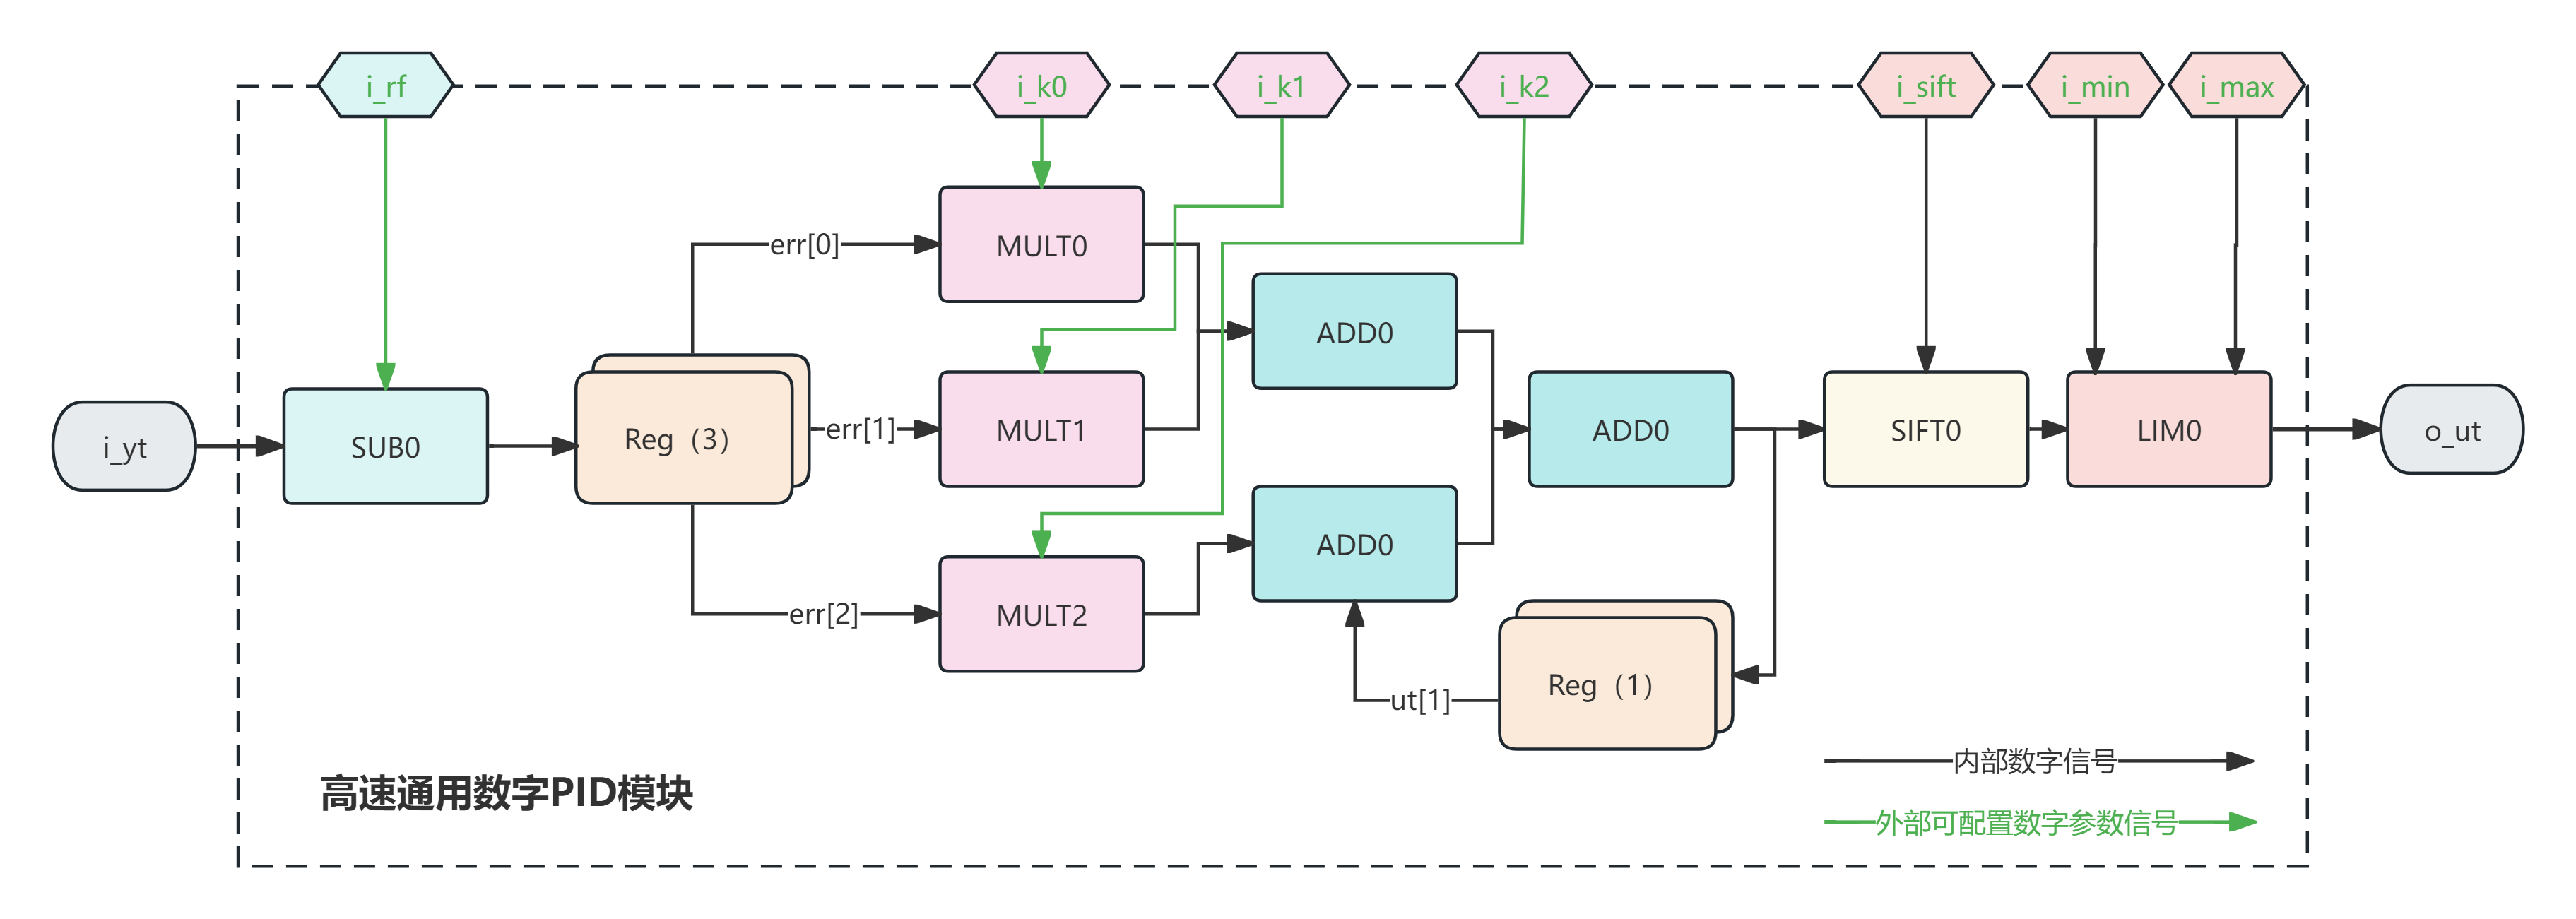
\includegraphics[width=1.0\linewidth]{rtmq/rtmq_pid_structure}
% \end{figure}

% 离散化后的PID表达式为:
% \begin{align}
%     u(n)=k_p e(n)+k_i\sum_{j=-}^{n}e(j)+k_d[e(n)-e(n-1)]\\
%     u(n-1)=k_p e(n-1)+k_i \sum_{j=0}^{n-1}e(j)+k_d [e(n-1)-e(n-2)]
% \end{align}

% 由上面两式可以导出:

% \begin{align}
%     \Delta u(n)=&u(n)-u(n-1)\\
%     =&k_0 e(n)+k_1 e(n-1)+k_2 e(n-2)
% \end{align}

% 其中$k_0=k_p+k_i+k_d,\ k_1=-k_p-2k_d,\ k_2=k_d$,这个式子被称为PID的增量算法。采用这种形式的好处是避免了计算PID原始表达式中的无限积分项。在这种增量式的方式下,PID的控制输出可以表达为:
% \begin{align}
%     u(n)=u(n-1)+\Delta u(n)=u(n-1)+k_0 e(n)+k_1 e(n-1)+k_2 e(n-2)\label{eq:increment_pid}
% \end{align}

% 按照上述式\eqref{eq:increment_pid}表示的增量式算法,数字PID实现的结构示意图如图\ref{fig:rtmq_pid_structure}所示。接口主要有参考$ref$、参数$k_0, k_1, k_2$、输出移位和限幅$shift, min, max$等可配置输入,反馈信号$y_t$等系统回路输入,以及$u_t$等系统控制输出。用到的器件包括加法器/减法器模块、乘法器模块、寄存器模块。

% \subsubsection[高速通用数字PID的FPGA实现]{高速通用数字PID的FPGA实现}

% % 增量式PID最终在FPGA中实现的结构图如图\ref{fig:digital_pid_structure_16bits}所示。

% 根据图\ref{fig:rtmq_pid_structure}所示的结构,可以在FPGA中实现硬件的PID。
% 其中主要涉及到的数字加法器、数字乘法器,分别采用的是超前进位加法器和Booth乘法器。对于高速时序电路,尤其是要满足与RTMQ的实时性匹配等相关需求,在开发过程中需要注意流水线的设置和对齐,最终的实现硬件框图如图\ref{fig:digital_pid_structure_16bits}所示,模块端口定义如表\ref{tb:rtmq_pid}所示。其硬件输出测试和仿真对比如\ref{fig:pid_compare}图所示。从图\ref{fig:pid_compare}中可见,在Vivado中实现的高速PID硬件电路在$k_i=1, k_d=1$的情况下经过大概1000ns后即可以将系统的输出稳定在参考值1000附近,与直接使用MATLAB进行数字PID仿真输出结果一致。

% \begin{table}
%     \centering
%     \caption[RTMQ系统外设高速通用PID模块端口定义]{RTMQ系统外设高速通用PID模块端口定义\label{tb:rtmq_pid}}    
%     \begin{tabular}{L{2.5cm}L{4cm}|L{2.5cm}L{4cm}}
%         \toprule
%         \multicolumn{2}{c|}{Input} & \multicolumn{2}{c}{Output} \\
%         \midrule
%         Port & Define & Port & Define\\
%         \hline
%         i\_clkp         & 系统时钟  & o\_ut[31:0] & PID输出结果 \\
%         i\_k0[15:0]     & PID参数k0 &  &  \\
%         i\_k1[15:0]     & PID参数k1 &  &  \\
%         i\_k2[15:0]     & PID参数k2 &  &  \\
%         i\_max[31:0]    & PID输出最高限幅 &  & \\
%         i\_min[31:0]    & PID输出最低限幅 &  & \\
%         i\_rstn         & PID重置信号 &  & \\
%         i\_rt[15:0]     & PID的系统输入信号 &  & \\
%         i\_shift[4:0]   & PID输出结果的偏移量 &  & \\
%         i\_yt[15:0]     & PID的反馈输入信号 &  & \\
%         \bottomrule
%     \end{tabular}
% \end{table}


% \begin{figure}
%     \centering
%     \caption[16位数字PID的FPGA实现结构图]{16位数字PID的FPGA实现结构图上\label{fig:digital_pid_structure_16bits}}
%     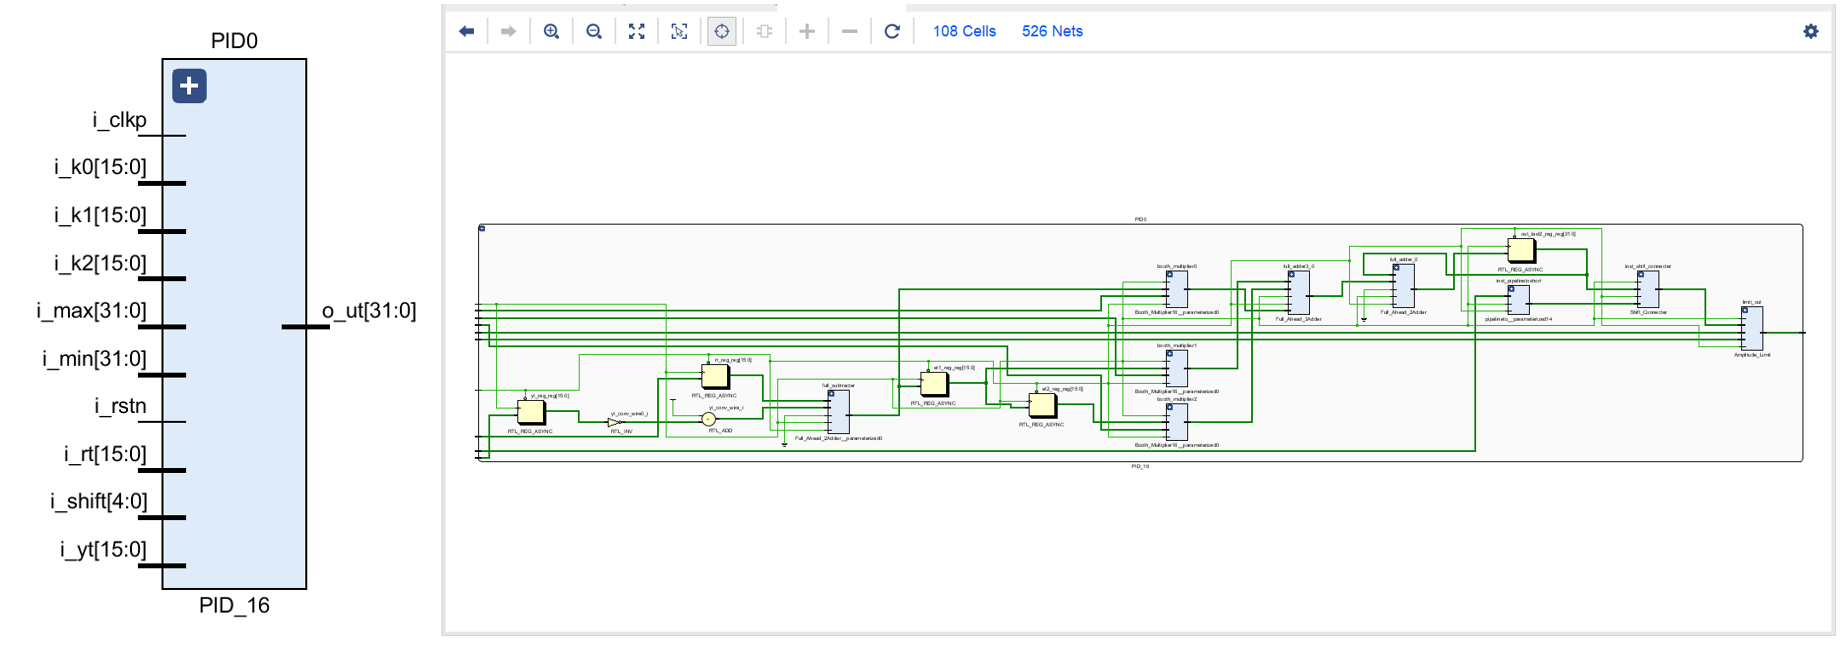
\includegraphics[width=1.0\linewidth]{rtmq/rtmq_pid}
% \end{figure}

% \begin{figure}
%     \centering
%     \caption[16位数字PID的FPGA实现结果与仿真结果对比]{16位数字PID的FPGA实现结果与仿真结果对比。初始系统输出和调节输出都为0,参考数值为1000,$k_i=1, k_d=1$,Vivado综合输出时长为3500ns,仿真持续时间为1000$T_c$(系统仿真迭代次数)。\label{fig:pid_compare}}
%     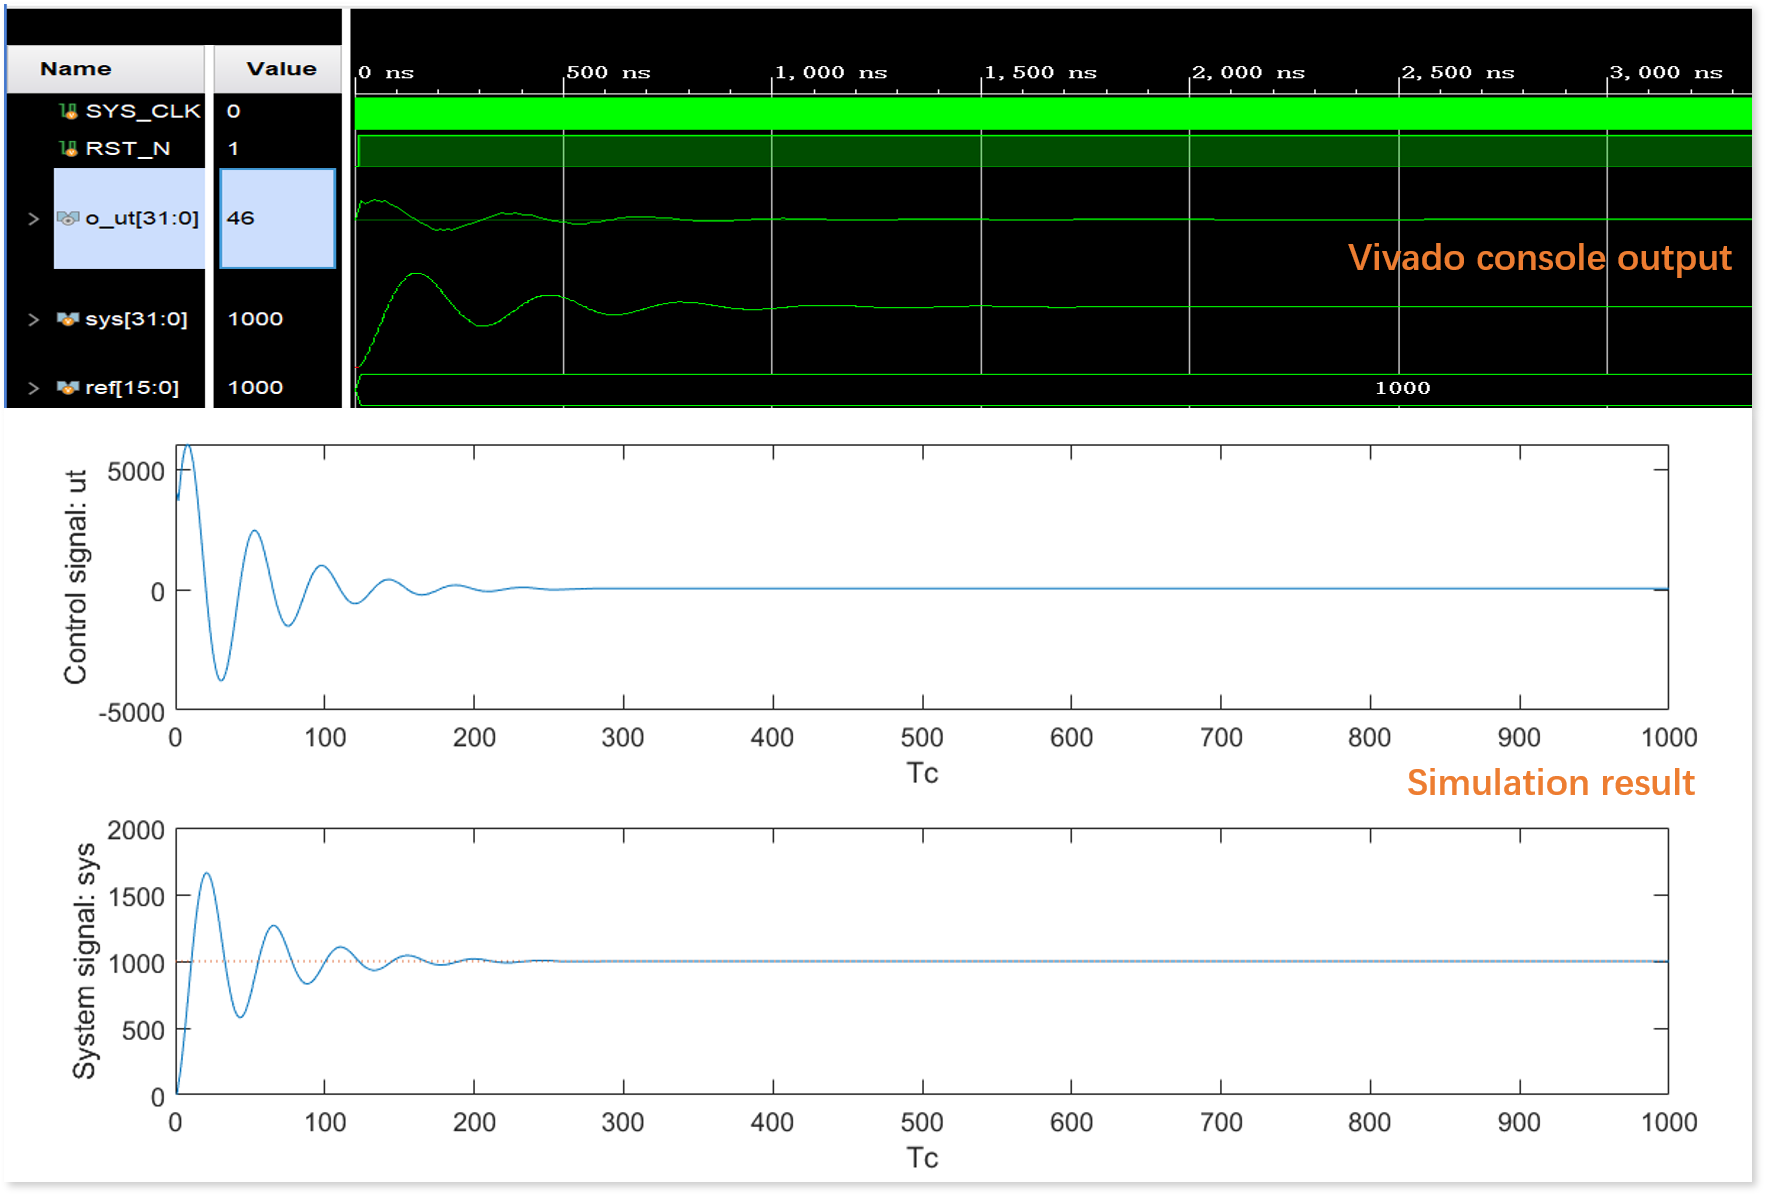
\includegraphics[width=1.0\linewidth]{rtmq/pid_compare}
% \end{figure}

% 整个PID控制器使用了一个减法器、三个加法器、三个乘法器和若干寄存器。图\ref{fig:digital_pid_structure_16bits}是一个16位输入的数字PID,它的输出是32位的,该实例模块总共包含9级流水线,工作频率可达200MHz以上。对更低或者更高位数的数字PID控制器,可以通过替换相应位数的加减运算和乘法模块,并调整相应的寄存器位宽来方便地得到。


% \subsection[高速通用数字IIR滤波器及其FPGA实现]{高速通用数字IIR滤波器及其FPGA实现\label{section:digital_iir}}
% % ============================================================================
% % =======================     高速数字滤波器    ===============================
% % ============================================================================


% 在量子计算的实现过程中,对于噪声的抗争从未停止。而对抗噪声的一种十分有效的方式就是使用各种各样的滤波器来对信号进行过滤以提高有用信号的质量。本质来讲,滤波器是一种选频装置,可以使信号中特定的频率成分通过,而极大地衰减其它频率成分。利用滤波器的这种选频作用,可以滤除干扰噪声或进行频谱分析。
% 当前实验系统中广泛出现滤波器为模拟滤波器,但是随着量子测控系统的数字化集成化进行逐步加深,在很多内部信号的处理上也有相当多的滤波需求,比如消除ADC芯片采样的噪声等。我们特别地在RTMQ系统板卡上实现了相匹配的高速通用数字IIR滤波器,来进一步实现对量子物理实验系统信号的控制和优化。


% \subsubsection[无限冲激响应滤波器IIR]{无限冲激响应滤波器IIR}
% 数字滤波器的基本原理是利用离散系统的特性对输入信号进行加工和处理,改变输入信号的频率特性,从而达到选频、提高信噪比、消除干扰等目的。数字滤波器一般由延迟单元、加法器、乘法器、寄存器等基本运算单元组成。不同类型的数字滤波器有不同的实现方法和应用领域。在通信、语音处理、图像处理、信号处理等领域,数字滤波器都有着广泛的应用。整个离子阱系统中很多模块都有滤波器的需求以获取更高质量的信号来控制量子比特。为此,整个RTMQ系统中需要实现数字滤波器以供系统设计和实现使用。

% 有限冲击响应滤波器(FIR滤波器)的冲激响应在有限时间内衰减为零,其输出仅取决于当前和过去的输入信号值。FIR滤波器在保证幅度特性的同时,很容易做到严格的线性相位特性。无限冲击响应滤波器(IIR滤波器)的冲激响应理论上应会无限持续,其输出不仅取决于当前和过去的输入信号值,也取决于过去的信号输出值。

% 有限冲击响应滤波器(FIR滤波器)的优点是具有线性相位、稳定性好、容易实现等,缺点是阶数较高时,运算量较大,对存储空间要求较高。无限冲击响应滤波器(IIR滤波器)的优点是阶数较低时,运算量较小,对存储空间要求较低,缺点是相位非线性、稳定性较差、设计复杂等。实际滤波器设计经验表明,实现相同形状的滤波效果,IIR滤波器所需的计算资源远小于FIR滤波器。鉴于硬件实现是对资源十分敏感的,因此我们选用IIR滤波器来进行实现。

% IIR滤波器的冲激响应理论上应会无限持续,其输出不仅取决于当前和过去的输入信号值,也取决于过去的信号输出值,用差分方程来表示一个滤波器,其表达式为:
% \begin{align}
%     y(n)=\sum_{k=1}^Na_ky(n-k)+\sum_{k=0}^Nb_kx(n-k)\label{eq:iir_filter}
% \end{align}


% 其中,$y(n)$表示输出信号,$x(n)$表示输入信号,$a_k$和$b_k$表示滤波器系数。本质上来说,IIR滤波器就是将输入和过去的输出按照某种方式加权计算获得最终输出结果的。对于一个给定阶数和数字位数的IIR滤波器,它的形状完全取决于系数$a_k$和$b_k$。因此,为了维持通用性,在硬件实现的过程中,我们应该把系数($a_k, b_k$)设计为可外部软件配置的。
% 以四阶为例,通用四阶IIR滤波器的结构框图如图\ref{fig:rtmq_iir_structure}所示,图中$a_0-a_3, b_0-b_3$为IIR滤波器的可配置系数,主要用到的模块有寄存器、乘法器、加法器等。
% \begin{figure}
%     \centering
%     \caption[IIR滤波器结构框图]{IIR滤波器结构框图。MULT:乘法器模块;Reg:寄存器模块;ADD:加法器模块;$i_filter, o_filter$:滤波器输入输出信号;$i_factor_a,i_factor_b$:IIR滤波器参数集合输入。\label{fig:rtmq_iir_structure}}
%     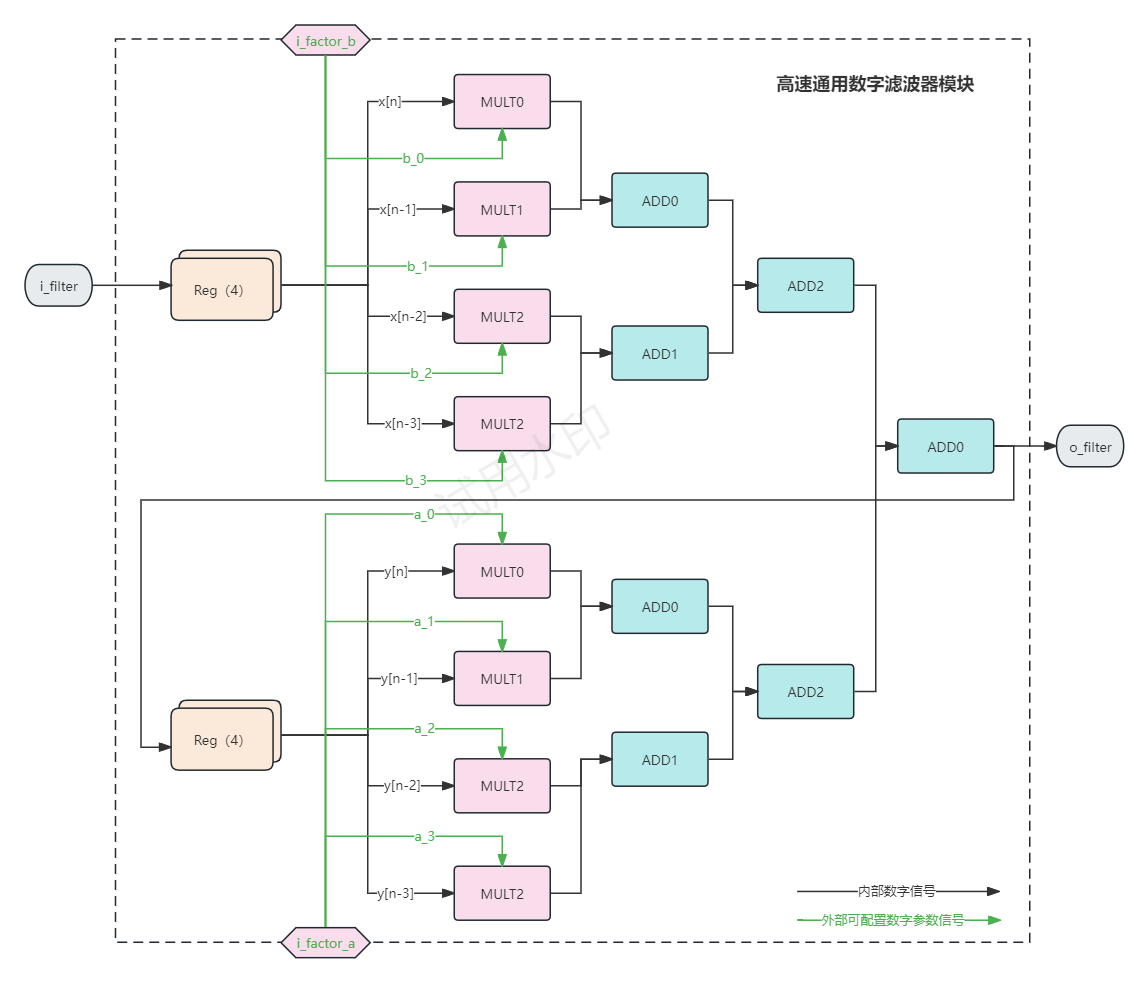
\includegraphics[width=1.0\linewidth]{rtmq/rtmq_iir_structure}
% \end{figure}


% \subsubsection[高速通用数字IIR滤波器的FPGA实现]{数字IIR滤波器的FPGA实现}

% 根据图\ref{fig:rtmq_iir_structure}给出的结构图和公式\eqref{eq:iir_filter},可以将其在FPGA中进行实现和验证。数字IIR滤波器在FPGA中的实现结果的结构图如图\ref{fig:iir_filter_vivado}所示,其模块端口定义如表\ref{tb:rtmq_iir_filter}所示。整体结构中插入了若干的流水线用于对齐$x(n)$和$y(n)$的时序。除此之外,流水线也被用于满足电路的时延要求。需要注意的是,由于上一时刻的输出结果$y(n-1)$需要参与到下一时刻的输出结果的计算中,因此从计算结果到迭代反馈之间仅能有一级流水线存在,否则输出结果就会出错。也即从乘法器输入到乘法器输出,以及加法器输入到加法器输出并反馈到乘法器输入这个回路中只能存在一级流水线。正因此,这个IIR滤波器无法工作在较高的频率上,需要在板上额外配置工作频率,该32位通用IIR滤波器设计在FPGA板上的工作频率为25MHz。


% \begin{table}
%     \centering
%     \caption[RTMQ系统外设高速通用PID模块端口定义]{RTMQ系统外设高速通用PID模块端口定义\label{tb:rtmq_iir_filter}}    
%     \begin{tabular}{L{3cm}L{3.5cm}|L{2.5cm}L{4cm}}
%         \toprule
%         \multicolumn{2}{c|}{Input} & \multicolumn{2}{c}{Output} \\
%         \midrule
%         Port & Define & Port & Define\\
%         \hline
%         i\_clkp             & 系统时钟 & o\_filter[31:0] & 滤波器输出 \\
%         i\_factor\_a[127:0] & 四阶滤波器参数a0[31:0]-a3[31:0] &  &  \\
%         i\_factor\_b[127:0] & 四阶滤波器参数b0[31:0]-b3[31:0] &  &  \\
%         i\_filter[31:0]     & 滤波器输入 &  &  \\
%         i\_rstn             & &  & \\
%         \bottomrule
%     \end{tabular}
% \end{table}


% \begin{figure}
%     \centering
%     \caption[IIR滤波器实现结果的结构图]{IIR滤波器实现结果的结构图(Vivado)\label{fig:iir_filter_vivado}}
%     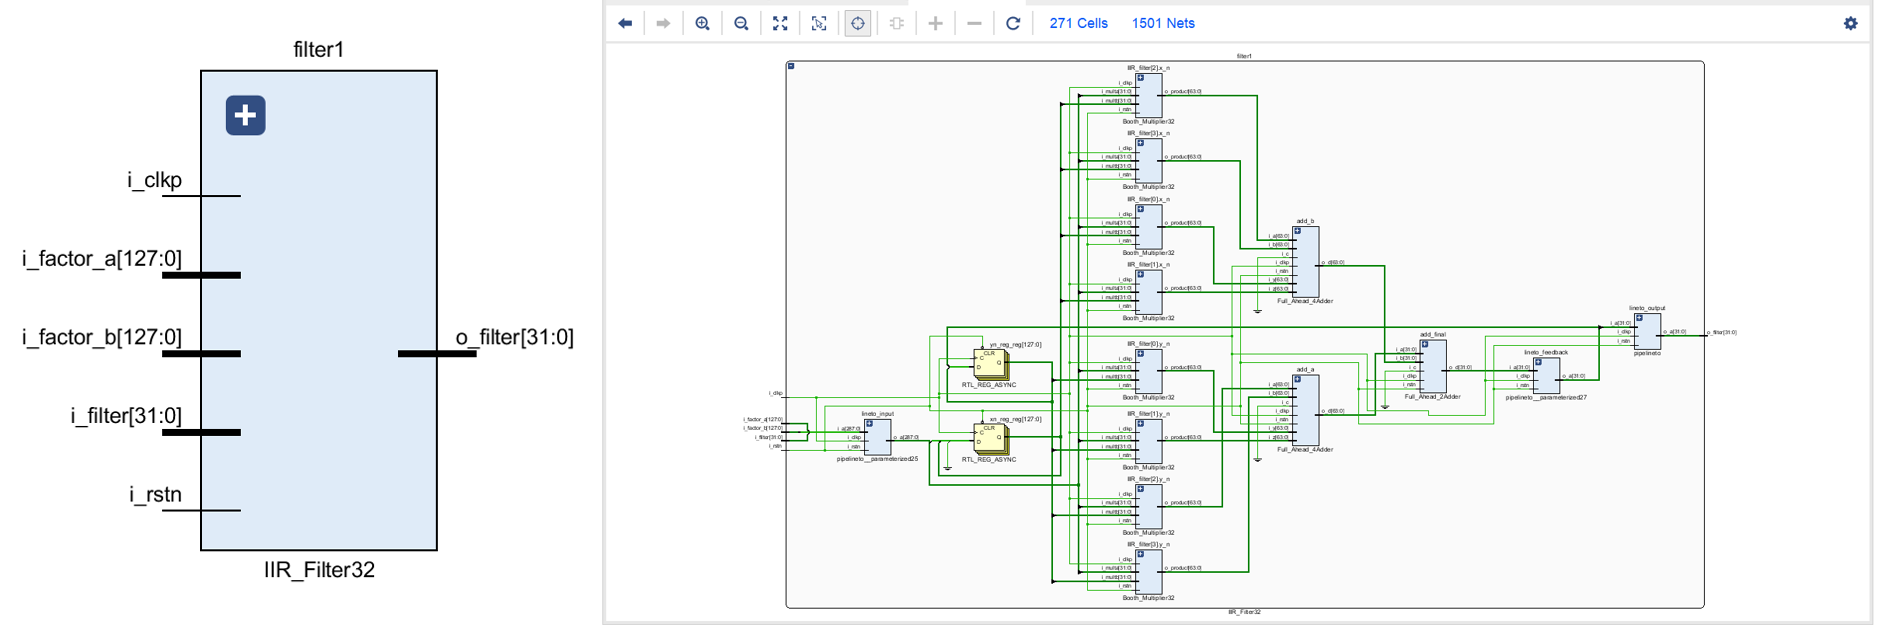
\includegraphics[width=1.0\linewidth]{rtmq/rtmq_iir_filter}
% \end{figure}




% \subsubsection[滤波器形状测量]{滤波器形状测量}
% 数字滤波器的形状设计可以采用MATLAB中的滤波器设计器来完成。在量子计算的实验系统中常常要应对的是高频信号噪声,低通滤波器是十分常见的需求,因此下面以低通滤波器为例进行说明。如图\ref{fig:filter_design_real1},通过MATLAB设计了一个截止频率在100kHz附近的巴特沃斯型迭代滤波器,结果为一个3阶的迭代滤波器,参数为:$a_0=16777216;
% a_1=-33470572;
% a_2=16693565;
% a_3=0;
% b_0=52;
% b_1=105;
% b_2=52;
% b_3=0$。可以看到设计的理论截止频率(100kHz)和数字滤波器实际的截止频率(13.17kHz)有较大的差异。其原因主要有两方面:1. 数字滤波器的设计本身实际上是对模拟滤波器的近似,因而结果不绝对准确;2. 实际在FPGA中的硬件滤波器运算位宽有限,爹地啊过程中存在截断效应;3. 对数据的表征不够精确,测试的过程中用到模数转换(16位)等中间数字过程。

% \begin{figure}
%     \centering
%     \caption[IIR滤波器设计仿真和实际测试结果]{IIR滤波器设计仿真和实际测试结果\label{fig:filter_design_real1}}
%     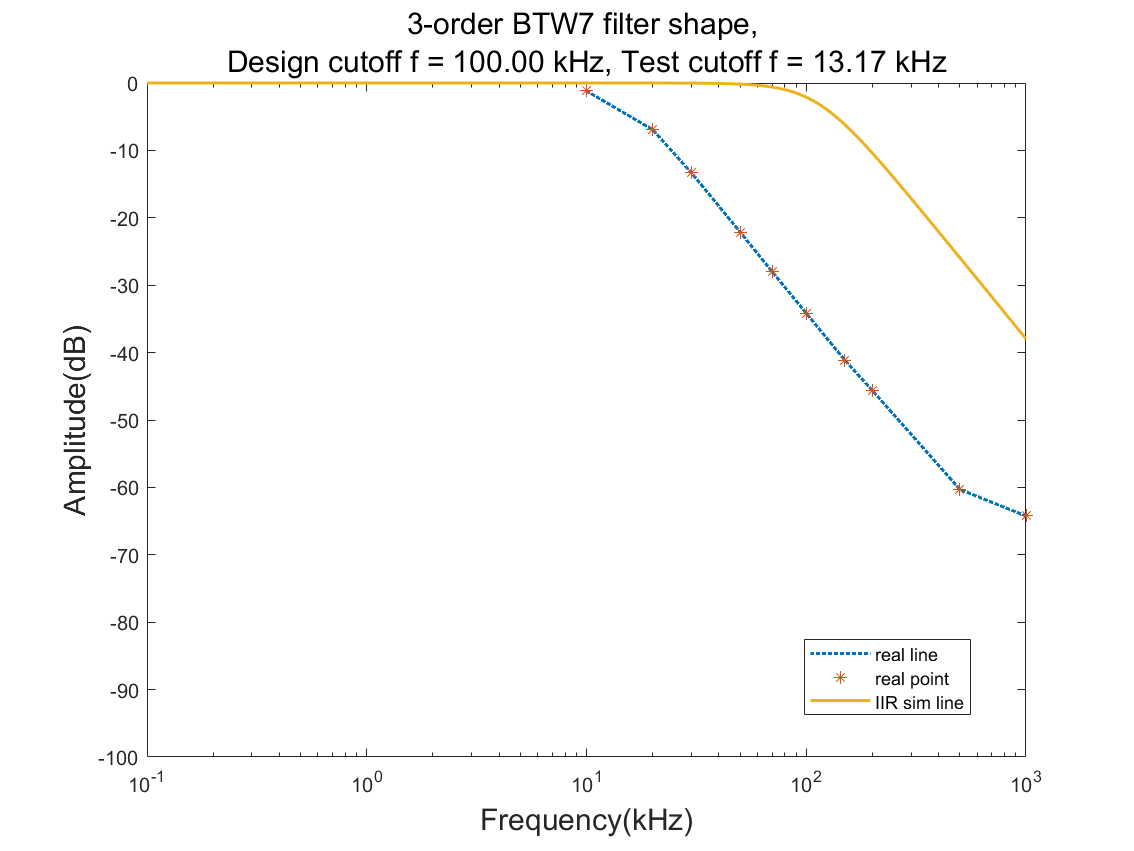
\includegraphics[width=1.0\linewidth]{rtmq/filter_design_real1}
% \end{figure}

% 在理论结果绘制中,对滤波器的结果进行类似FPGA硬件中的人工截断,得到的模拟结果如图\ref{fig:filter_design_real2}所示。可以看到此时理论设计的截止频率结果与实际硬件数字PID的截止频率结果变得更加接近了。尽管仍然存在一定的差异,已经可以给出比较有意义的指导信息了。整体上来看,硬件实现的数字滤波器在配置为低通滤波器的时候带宽会被压窄。因此如果需要100kHz的带宽,则需要在设计时适当放大这个带宽需求。最终实际的滤波器带宽可以通过测量来进一步验证是否符合使用要求,如果不符合则可以重新设计和测试。值得一提的是,在实现了通用的硬件IIR滤波的基础上,重新设计和配置$a_0-a_3, b_0-b_3$等参数是十分方便快捷的,仅需更改可配置寄存器的值即可。

% \begin{figure}
%     \centering
%     \caption[IIR滤波器考虑截断的仿真和实际测试结果]{IIR滤波器考虑截断的仿真和实际测试结果\label{fig:filter_design_real2}}
%     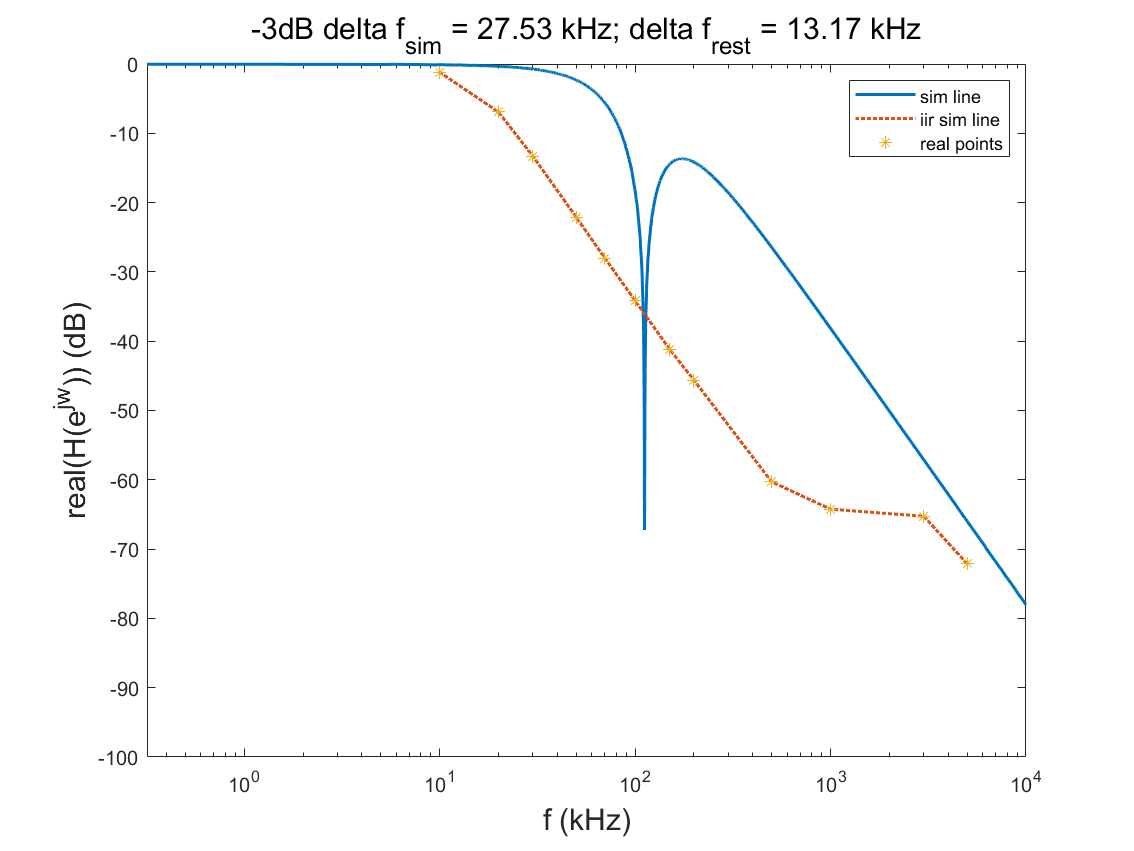
\includegraphics[width=1.0\linewidth]{rtmq/filter_design_real2}
% \end{figure}

% % IIR滤波器形状测量如图\ref{fig:iir_filter_shape}所示。
% % \begin{figure}
% %     \centering
% %     \caption[IIR滤波器设计仿真和不同参数下测试结果]{IIR滤波器设计仿真和不同参数下测试结果\label{fig:iir_filter_shape}}
% %     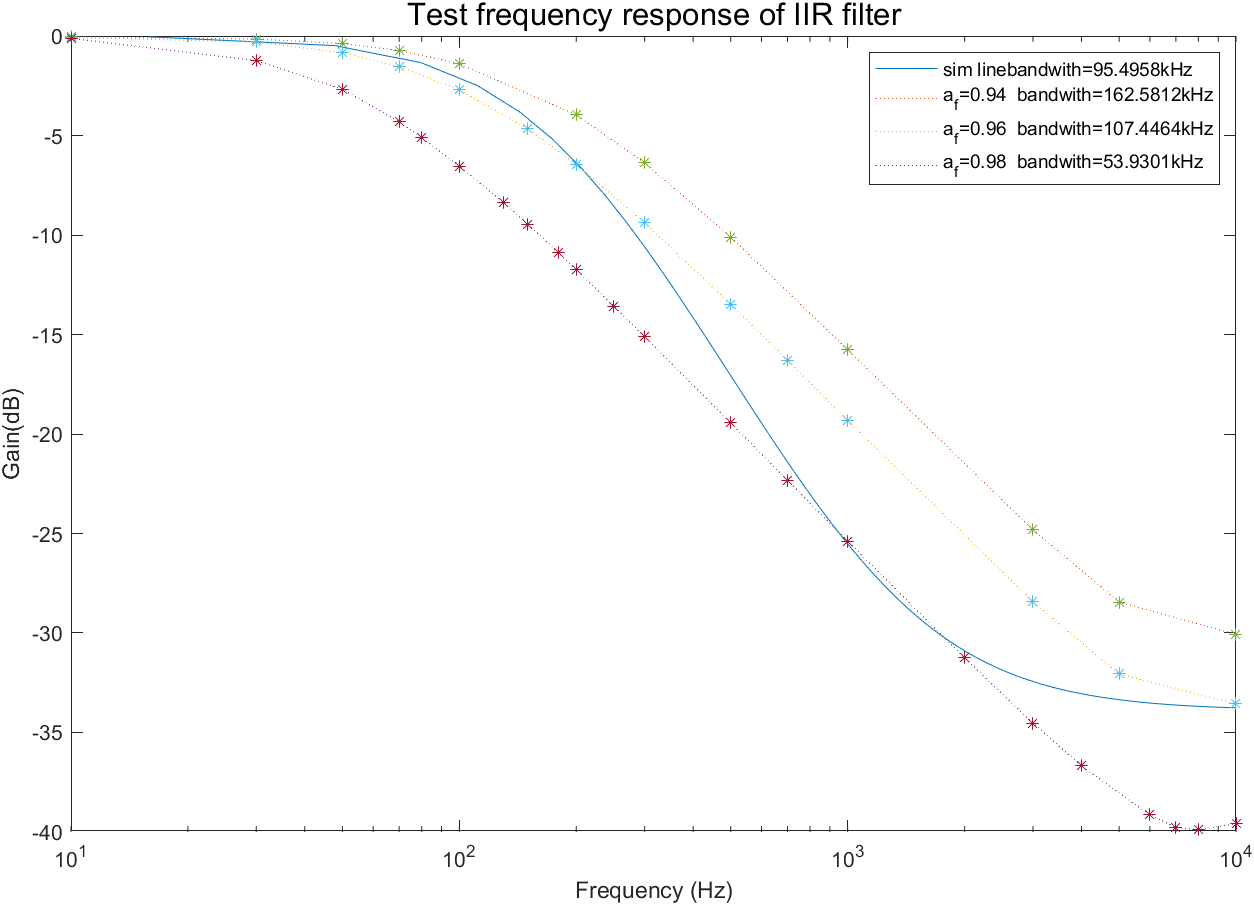
\includegraphics[width=1.0\linewidth]{rtmq/iir_filter_shape}
% % \end{figure}


% \newpage


\section[章末小结]{章末小结}

在量子计算实验系统中,测控系统占据着十分关键的位置。对于离子阱量子计算系统来说,它将系统中涉及到的电学、光学、真空等其余各个子系统联系起来,给出各类光电信号对离子比特进行操控以实现量子计算。为了满足量子计算发展过程中日益增高的量子测控需求,本章介绍了一套强实时、可拓展、分布式的用于量子物理实验的实时微系统——RTMQ。RTMQ是专为量子物理实验设计的一套测控系统方案,它包含了一种专门设计的用于满足实时信息处理的微处理器架构以及配套的指令集,此外还有服务于节点拓展的通信链路系统。

本章首先明确了量子测控系统的两个主要挑战:信息处理实时性和大规模拓展性,并分析了现有传统以及量子测控系统的优缺点。
随后介绍了RTMQ量子测控系统的整体架构以及每个RTMQ节点的内部模块,同时也给出了RTMQ的测控板实现及主要功能器件说明,
还有微处理器的核心模块的流控制器、计时器、算术逻辑单元等三个子模块的FPGA实现。
接着描述了RTMQ微处理器所配套设计的指令集,介绍了指令集的汇编指令格式以及其I类和A类两类指令的操作码、指令功能和编码方式,并给出了其时序控制结构实例。
值得关注的是,从它的指令集中可以看到RTMQ测控系统系统是支持板上运算和信息处理的,这是与其它依靠时序发生器构成的测控系统本质不同的地方和优势所在。这些处理包括逻辑运算和算术运算,构成了一个微处理器。而RTMQ系统的微处理器从架构上与CPU有着本质的不同,虽然牺牲了些运算效率,RTMQ的数据处理是严格实时的。这种处理器架构同样也具有拓展性和灵活性,我们可以方便地为它拓展和定义多种运算方式,也可以为其添加外设模块等,以适应更多更复杂任务的需求。对RTMQ量子测控系统的理解为后续设计测控板硬件及离子阱量子计算重要子系统的搭建和测试(第\ref{section:implementation}章)打下了基础。
